% !TEX root = ../main.tex



% EDITS TO BE MADE:
% 1- Different market participants would have different preference about various markets. Which one is best for which? Jeremy in proposal: could be a chart
% 2- Add a subsection on latency
% 3- For enqueue and dequeue performance tests, justify why you picked 50 integers

\section{Introductory Remarks}

There are three main approaches to arranging a trade~\cite{Har03}. In a \emph{quote-driven} market, a dealer uses its own inventory to offer a price for buying or selling an asset. In a \emph{brokered exchange}, a broker finds a buyer and seller. In an \emph{order-driven} market, offers to buy (\emph{bids}) and sell (\emph{offers}/\emph{asks}) from many traders are placed as orders in an order book. Order-driven markets can be \emph{continuous}, with buyers/sellers at any time adding orders to the order book (\emph{makers}) or executing against an existing order (\emph{takers}); or they can be \emph{called}, where all traders submit orders within a window of time and orders are matched in a batch (like an auction). 

Conventional financial markets (\eg NYSE, NASDAQ) use both continuous time trading during open hours, and a call market before and during open hours to establish an opening price and a closing price. After early experiments at implementing continuous time trading on Ethereum (\eg EtherDelta, OasisDEX), it was generally accepted that conventional trading is infeasible on Ethereum for performance reasons. Centralized exchanges continued their predominance, while slowly some exchanges moved partial functionality on-chain (\eg custody of assets) while executing trades off-chain. 

A clever quote-driven alternative, called an automatic market maker (AMM), was developed that only requires data structures and traversals with low gas-complexity. This approach has undesirable price dynamics (\eg market impact of a trade, slippage between the best bid/ask and actual average execution price, \etc) which explains why there is no Wall Street equivalent, however it is efficient on Ethereum and works `good enough' to attract trading. First generation AMMs provide makers (called liquidity providers) with no ability to act on price information---they are uninformed traders that can only lose (called impermanent loss) on trades but make money on fees. Current generation AMMs (\eg Uniswap v3) provided informed makers with a limited ability (called concentrated liquidity) to act on proprietary information~\cite{Park21} without breaking Ethereum's performance limitations. Ironically, the logical extension of this is a move back to where it all started---a full-fledged order-driven exchange that allows informed makers the fullest ability to trade strategically.



%For better or worse, blockchain technologies like Ethereum have dramatically lowered the barrier to entry for developing and deploying financial technology. New tokens have been launched with a few clicks of a user interface, and large investment infrastructures have been developed and deployed with little regulatory oversight. Blockchain exchange services allow order-based trading of digital currencies, tokens, and other digital assets. Such exchanges are key components to blockchain-based economic activity.

%Financial regulators seek to provide consumer protection during the issuing and trading of financial products and assets. They are concerned by their limited ability to intervene when trading is conducted on decentralized networks that, like Ethereum, run on the open internet. Order-driven trading can happen fully `on-chain' and this was experimented within the early days of Ethereum, but it has been largely abandoned for performance reasons in favor of running on centralized servers. More specifically, the core functionality is performed off-chain (\eg matching orders) while other aspects (\eg loading accounts, order cancellation) might be performed on-chain. In this world, company names, employees, addresses, and publicly addressable servers all provide regulatory hooks.


% Final camera-ready
% JC: Our research group is actively collaborating with our jurisdiction's (Quebec, Canada) financial regulator, the Autorité des Marchés Financiers (AMF), to help them forecast how trading can be impacted by blockchain technology.

%Our research group is actively collaborating with our jurisdiction's financial regulator (name withheld for anonymity) to help them forecast how trading can be impacted by blockchain technology. This paper addresses their concerns about the feasibility of a `worst-case scenario' where a trading platform is anonymously deployed on a public blockchain, like Ethereum, and runs autonomously without any further intervention from an externally visible entity. Such a design appears feasible but is considered too slow. Together, we agreed it is a very good time to do a deep dive into understanding precisely \textit{how slow} for the following reasons: (1) public blockchains are becoming faster (both in theory and in practice) providing future efficiency gains for on-chain trading, (2) demand for on-chain trading is exemplified by the recent popularity of dealer quote-based trading like Uniswap and Curve Finance (reviewed below), and (3) stablecoins have become popular and allow on-chain trading with pricing in USD, alleviating another regulatory hook: the need for platforms to maintain traditional accounts for holding governmental currency and interfacing with the banking system.

\textbf{Contributions.} In this paper, we experiment with on-chain markets to understand in detail if they remain infeasible on Ethereum and what the limiting factors are. Some highlights from our research include answering the following questions:
\begin{itemize}
\item What type of exchange has the best properties on balance? (A call market.)
\item How many orders can be processed on-chain? (Upper-bounded by 152 per block.)
\item How much efficiency can be squeezed from diligently choosing the best data structures? (Somewhat limited: turn 38 trades into 152.)
\item To what extent can we mitigate front-running attacks? (Almost entirely.)
\item Can we stop the exchange's storage footprint on Ethereum from bloating? (Yes, but it is so expensive that it is not worth it.)
\item Are on-chain order books feasible on layer 2? (Yes! Optimistic roll-ups reduce gas costs by 99.88\%.)
\item Which aspects of Ethereum were encountered that required deeper than surface-level knowledge to navigate? (Optimizing gas refunds, Solidity is not truly object-oriented, miner extractable value (MEV) can be leveraged for good, \textblue{add more?})
\item How hard is an on-chain exchange to regulate? (The design leaves almost no regulatory hooks beyond miners (and sequencers on layer 2).)
\end{itemize}


 % design and implementation with Solidity---a high-level programming language for Ethereum that is syntactically similar to Java.
 
 % We choose Ethereum as a hostile environment for an order book: Ethereum is fully decentralized (hardest to regulate), network participation is open to anyone on the internet (strongest adversarial model), and, as a result, it is slow (a lower-bound benchmark). Generally, if an application is feasible on Ethereum, it will also be feasible and only run faster on a private (or permissioned) blockchain (\eg Hyperledger), which is a blockchain operated by authorized network nodes only, generally visible to regulators.

% Our proof of concept, \cm, is an extensible base class suitable for experiments. \cm is designed from a security perspective: users only trust their assets to \cm's auditable code (non-custodial) and not to a third party, all operations are transparent, and we nearly eliminate the ability for adversarial network nodes to profit from front-running orders (see Section~\ref{sec:front} for in-depth front-running analysis). In fact, we believe we are the first to design a decentralized application that actually leverages front-running (\ie miner extractable value~\cite{daian2019flash}) for the benefit of the system (see Section~\ref{sec:close}).

%While Solidity and its compiled bytecode is like many common programming languages, it also has quirks that require experimentation to best optimize performance (\eg factoring in the gas costs of operations, gas refunds, limits to Solidity's object-oriented design, clearing mappings, \etc). We test five priority queues---the core data structure of the call market---and various options for cleaning up our data once finished with it. The bottom line is that the current benchmark for a \cm-esque design is in the low hundreds of trade executions per block on Ethereum today. This positions \cm as a feasible design for only a narrow set of markets today (low liquidity, small number of traders) which is good news for regulators. A broader consequence of our research is that any on-chain application that requires the traversal of hundreds of elements in a data structure in a single transaction is not feasible on Ethereum today.

%We also speculate that Ethereum is likely to improve vastly in the coming years and we demonstrate one avenue for improvement through `roll-ups'~\cite{kalodner2018arbitrum} which reduce the gas costs of \cm by more than 99.9\%. While roll-ups are not fully on-chain and introduce new network participants, the roll-up architecture is still concerning to regulators because the participants (called validators) are not directly reachable by users; they only watch the Ethereum state and interact directly with Ethereum.

% = = = = = = = = = = = = = = = = = = = = = = = = = = = = = = = = = = = = = = = = = =
% = = = = = = = = = = = = = = = = = = = = = = = = = = = = = = = = = = = = = = = = = =
% = = = = = = = = = = = = = = = = = = = = = = = = = = = = = = = = = = = = = = = = = =

\section{Preliminaries}

\subsection{Ethereum}

We assume the reader is familiar with the following concepts: blockchain technology; smart contracts and decentralized applications (DApps) on Ethereum; how Ethereum transactions are structured, broadcasted, and finalized; the gas model including the gas limit (approximately 11M gwei at the time of our experiments) per block. A \textbf{gas refund} is a more esoteric subject (not covered thoroughly in any academic work to our knowledge) that we use heavily in our optimizations. Briefly, certain EVM operations (\texttt{SELFDESTRUCT} and \texttt{SSTORE 0}) cost negative gas, with the follow caveats: the refund is capped at 50\% of the total gas cost of the transaction, and (2) the block gas limit applies to the pre-refunded amount (\ie a transaction receiving a full refund can cost up to 5.5M gas with an 11M limit). We provide full details of all of these topics in Appendix~\ref{app:ethback}. 

\subsection{Trade Execution Systems}

% !TEX root = ../main.tex
 \newcolumntype{P}[1]{>{\centering\arraybackslash}p{#1}}
% = = = = = = = = = = = = = = = = = = = = =Call market operations Table = = = = = = = = = = = =  = = = = = =  %
\begin{table}[t]
%\setlength{\tabcolsep}{0.7\tabcolsep}% Shrink \tabcolsep

\centering
\scriptsize
%\begin{tabular}{|>{\centering}m{3cm} |>{\centering}m{3cm} |>{\centering}m{3cm} |>{\centering}m{4cm} |}
\begin{tabular}{|c|c|c|c|}

\hline
\textbf{Exchange Platform}			 &\textbf{Description}   				& \textbf{Advantages}      				& \textbf{Disadvantages}                   \\ \hline

% = = = = = = = = = = = = = = = = = = = = = = = = = = = = = = = = = = = = = = = = = = = = = = = = = = = = = = = = == = = = = = = = = = = = = = = = = = = = = = = = = = = = = = = = = = = = = = = = = = = = = = = = = = = == = = = = = = = = = = = = = = = = = = = = = = = = == = = = = =%
\multirow{4}{*}{\shortstack{Centralized \\Exchanges}}                            & \multirow{4}{*}{\shortstack{Exchange acts as a \\trusted third party\\ between traders}} 	& High Liquidity			& Third party custodian				\\  
											&																		& High trade performance		& Low security				\\ 
											 &																		& Low price slippage		& No instant settlement	 		\\
											 &																		& Easy to regulate			& Server downtime							\\ \hline
					
% = = = = = = = = = = = = = = = = = = = = = = = = = = = = = = = = = = = = = = = = = = = = = = = = = = = = = = = = == = = = = = = = = = = = = = = = = = = = = = = = = = = = = = = = = = = = = = = = = = = = = = = = = = = == = = = = = = = = = = = = = = = = = = = = = = = = == = = = = =%
\multirow{6}{*}{\shortstack{On-chain \\Order Books}}                         		& \multirow{6}{*}{\shortstack{Exchange operates\\fully \\on-chain as coded}}	& High security							&	\\
												&																		& Non-custodial						& 					\\
												&																		& No trusted third party					& Low trade performance						\\
												&																		& Fully Autonomous						&Hard to regulate			\\
												&																		& No Impermanent Loss					&					\\
												&																		& Low price slippage					&					\\ \hline
																									
% = = = = = = = = = = = = = = = = = = = = = = = = = = = = = = = = = = = = = = = = = = = = = = = = = = = = = = = = == = = = = = = = = = = = = = = = = = = = = = = = = = = = = = = = = = = = = = = = = = = = = = = = = = = == = = = = = = = = = = = = = = = = = = = = = = = = == = = = = =%
\multirow{5}{*}{\shortstack{On-chain \\Dealers} }                     	 & \multirow{5}{*}{ \shortstack{A dealer uses its \\own inventory to offer \\a price for assets \\being traded}}	& High security				& 				\\										
											&																						& Non-custodial			&  Impermanent Loss\\
											&																						& No trusted third party		&	High price slippage				\\
											&																						& Fully Autonomous			&	 No support for limit orders			\\
											&																						& High performance			&					\\ \hline
																									

% = = = = = = = = = = = = = = = = = = = = = = = = = = = = = = = = = = = = = = = = = = = = = = = = = = = = = = = = == = = = = = = = = = = = = = = = = = = = = = = = = = = = = = = = = = = = = = = = = = = = = = = = = = = == = = = = = = = = = = = = = = = = = = = = = = = = == = = = = =%
\multirow{3}{*}{\shortstack{Hybrid\\ Designs}}                            &  \multirow{3}{*}{\shortstack{Exchange operates \\partially on-chain}}  								& High trade performance				& Low security										\\
									&																									& Easy to regulate					& Server downtime \\
									&																									& Non-custodial 					& \shortstack{Uncertain fair execution}	\\ \hline
% = = = = = = = = = = = = = = = = = = = = = = = = = = = = = = = = = = = = = = = = = = = = = = = = = = = =  %
\end{tabular}
\caption{ A simple comparison among different trade execution systems.
\label{tab:eval2}}
\end{table}

% = = = = = = = = = = = = = = = = = = = = = = = = = = = = = = = = = = = = = = = = = = = = = = = = = = = =  %

Table~\ref{tab:eval2} illustrates various trade execution systems and summarizes their advantages and disadvantages. Appendix~\ref{app:markets} provides a full justification for the table. Briefly, fully decentralized, on-chain exchanges require the lowest trust, provide instant settlement, and have transparent trading rules that will always execute correctly. Front-running attacks (see Section~\ref{sec:front} for a very thorough discussion) are a weakness inherent in blockchains that require specific mitigation.  

\subsection{Related Work}

Call markets are studied widely in finance and provide high integrity prices (\eg closing prices that are highly referenced and used in derivative products)~\cite{HS04,PS03,FH21}. They can also combat high frequency trading~\cite{budish2015high,aquilina2020quantifying}. An older 2014 paper~\cite{clark2014decentralizing} on the `Princeton prediction market'~\cite{Bra13} show that call markets  mitigate most blockchain-based front-running attacks present in an on-chain continuous-trading exchange as well as other limitations: block intervals are slow and not continuous, there is no support for accurate time-stamping, transactions can be dropped or reordered by miners, and fast traders can react to submitted orders/cancellations when broadcast to network but not in a block and have their orders appear first. The paper does not include an implementation, was envisioned as running on a custom blockchain (Ethereum was still in development in 2014) and market operations are part of the blockchain logic. 

The most similar academic work to this paper is the Ethereum-based periodic auction by Galal \etal~\cite{galalpublicly} and the continuous-time exchange TEX~\cite{khalil2019tex}. As with us, front-running is a main consideration of these works. In a recent SoK on front-running attacks in blockchain~\cite{eskandari2019sok}, three general mitigations are proposed: confidentiality, sequencing, and design. Both of these papers use confidentiality over the content of orders~(\cf \cite{TP07,YSLT10,TW12,cartlidge2019mpc,massacci2018futuresmex}). The main downside is that honest traders cannot submit their orders and leave, they must interact in a second round to reveal their orders. The second mitigation approach is to sequence transactions according to some rule akin to first-in-first-out~\cite{kelkar2020order,Kla20}. These are not available for experimentation on Ethereum yet (although Chainlink has announced an intention\footnote{A. Juels. \href{https://blog.chain.link/chainlink-fair-sequencing-services-enabling-a-provably-fair-defi-ecosystem/}{blog.chain.link}, 11 Sep 2020.}). The third solution is to design the service in a way that front-running attacks are not profitable---this is the approach with \cm which uses \textit{no cryptography} and is \textit{submit-and-go} for traders. A detailed comparison of front-running is provided in Section~\ref{sec:front}. Our paper also emphasizes implementation details: Galal \etal do not provide a full implementation, and TEX uses both on-chain and off-chain components, and thus does not answer our research question of how feasible an on-chain order book is.


% = = = = = = = = = = = = = = = = = = = = = = = = = = = = = = = = = = = = = = = = = =
% = = = = = = = = = = = = = = = = = = = = = = = = = = = = = = = = = = = = = = = = = =
% = = = = = = = = = = = = = = = = = = = = = = = = = = = = = = = = = = = = = = = = = =


\section{Call Market Design}

% !TEX root = ../main.tex

% = = = = = = = = = = = = = = = = = = = = =Call market operations Table = = = = = = = = = = = =  = = = = = =  %
\begin{table}[t]
%\setlength{\tabcolsep}{0.7\tabcolsep}% Shrink \tabcolsep

\centering
\scriptsize
\begin{tabular}{|>{\centering}m{2.2cm} |>{\centering\arraybackslash}m{7cm}|}%{|c|c|}

\hline
\multicolumn{1}{|c|}{\textbf{Operation}} & \multicolumn{1}{c|}{\textbf{Description}}                            			\\ \hline

% = = = = = = = = = = = = = = = = = = = = = = = = = = = = = = = = = = = = = = = = = = = = = = = = = = = =  %
	depositToken()                           & Deposits ERC20 tokens in \cm smart contract \\ \hline
% = = = = = = = = = = = = = = = = = = = = = = = = = = = = = = = = = = = = = = = = = = = = = = = = = = = =  %
	depositEther()                           	& Deposits ETH in \cm smart contract                        			 \\ \hline
% = = = = = = = = = = = = = = = = = = = = = = = = = = = = = = = = = = = = = = = = = = = = = = = = = = = =  %
	openMarket()                             & Opens the market                                                    					 \\ \hline
% = = = = = = = = = = = = = = = = = = = = = = = = = = = = = = = = = = = = = = = = = = = = = = = = = = = =  %
	closeMarket()                            & Closes the market and processes the orders       \\ \hline
% = = = = = = = = = = = = = = = = = = = = = = = = = = = = = = = = = = = = = = = = = = = = = = = = = = = =  %
	submitBid()                              & Inserts the upcoming bids inside the priority queue   \\ \hline
% = = = = = = = = = = = = = = = = = = = = = = = = = = = = = = = = = = = = = = = = = = = = = = = = = = = =  %
	submitAsk()                              & Inserts the upcoming asks inside the priority queue  \\ \hline
% = = = = = = = = = = = = = = = = = = = = = = = = = = = = = = = = = = = = = = = = = = = = = = = = = = = =  %
	claimTokens()                           & Transfers tokens to the traders                       			\\ \hline
% = = = = = = = = = = = = = = = = = = = = = = = = = = = = = = = = = = = = = = = = = = = = = = = = = = = =  %
	claimEther()                             & Transfers ETH to the traders                       			\\ \hline
% = = = = = = = = = = = = = = = = = = = = = = = = = = = = = = = = = = = = = = = = = = = = = = = = = = = =  %
\end{tabular}
\caption{Primary operations of \cm smart contract.
\label{tab:cm_functions}}
\end{table}

% = = = = = = = = = = = = = = = = = = = = = = = = = = = = = = = = = = = = = = = = = = = = = = = = = = = =  %

For our experiments and measurements, we implement an exchange from scratch. \cm is a call market that will open for a specified period of time during which it will accept a capped number of orders (\eg 100 orders---parameterized so that all orders can be processed), and these orders are added to a priority queue (discussed in Section~\ref{sec:pq} ). Our vision is the market would be open for a very short period of time, close, and then reopen immediately (\eg every other block). \cm is open source and written in 336 lines (SLOC) of Solidity plus the priority queue (\eg we implement 5 variants, each around 300 SLOC). We tested it with the Mocha testing framework using Truffle~\cite{TruffleO71:online} on Ganache-CLI~\cite{GanacheT25:online} to obtain our performance metrics. Once deployed, the bytecode of \cm is 10,812 bytes plus the constructor code (6,400 bytes) which is not stored. The Solidity source code for \cm and Truffle test files are available in a GitHub repository.\footnote{Github: Link removed for anonymity.} We have also deployed \cm on Ethereum's testnet Rinkeby with flattened (single file) source code of just the \cm base class and priority queue implementations. It is visible and can be interacted with here: \href{https://rinkeby.etherscan.io/address/0x0d91de29c531d074853a5cef7cf9dfeb9c6ec4e0}{[etherscan.io]}. We cross-checked for vulnerabilities with \textit{Slither}\footnote{https://github.com/crytic/slither} and \textit{SmartCheck}\footnote{https://tool.smartdec.net} and it only fails some `informational' warnings that are intentional design choices (\eg a costly loop). All measurements assume a block gas limit of $11\,741\,495$ and 1 gas $=$ 56 Gwei.\footnote{EthStats (July 2020): \url{https://ethstats.net/}} Table~\ref{tab:cm_functions} summarizes \cm's primary operations.

%\textblue{Figuremindmap represents a design  landscape and extensions.}

%is an extensible base class that is still functional without any extensions. 
%
%Later in Section~\ref{sec:close}, we discuss the options for who closes/reopens the market. We keep the design simple by not allowing cancellations which require a second transaction and front-running attacks apply to cancellation orders~\cite{eskandari2019sok}. As markets are relatively short-lived, orders simply expire when the market call period ends.
%
%Another simplifying assumption is to implement a \textit{collateralized} call market. We assume all trades are between ETH and an ERC20 token, all orders are pre-funded in the contract with ETH (for bids) and tokens (for asks), and once ETH or tokens are committed to an order, they cannot be withdrawn until the market closes. This ensures all executed orders clear and settle (\ie no defaults on payment or delivery).

% Volume of 1
% Ties?

% = = = = = = = = = = = = = = = = = = = = = = = = = = = = = = = = = = = = = = = = = =
% = = = = = = = = = = = = = = = = = = = = = = = = = = = = = = = = = = = = = = = = = =
% = = = = = = = = = = = = = = = = = = = = = = = = = = = = = = = = = = = = = = = = = =

\subsection{Priority Queues}\label{sec:pq}

%% = = = = = = = = = = = =Operations for a generic Priority Queue Table = = =  = = = = = = = = = = = %
\begin{table}[t]
\centering
\begin{tabular}{|c|c|}
\hline

\textbf{Operation}   & \textbf{Description}    \\ \hline

% = = = = = = = = = = = = = = = = = = = = = = = = = = = = = = = = = = = = = = = = = = = = = = = = %
	\textbf{Enqueue()}       	& Inserts an element into the priority queue                        \\ \hline
	\textbf{Dequeue()}		& Removes and returns the highest priority element 		\\ \hline
	\textbf{isEmpty()}			& Checks if the priority queue is empty 					\\ \hline
% = = = = = = = = = = = = = = = = = = = = = = = = = = = = = = = = = = = = = = = = = = = = = = = =  %

\end{tabular}
\caption{\footnotesize{Operations for a generic priority queue.}
\label{tab:PQ_API}}
\end{table}
% = = = = = = = = = = = = = = = = = = = = =  = = = = = = = = = = =  = = = = = = = = = == = = =  = =%

In designing \cm within Ethereum's gas model, performance is the main bottleneck. For a call market, closing the market and processing all the orders are the most time-consuming steps. Assessing which data structures will perform best is hard (\eg gas refunds, a relatively cheap mapping data structure, only partial support for object-oriented programming) without actually deploying and evaluating several variants.

We first observe that orders are executed in order: highest to lowest price for bids, and lowest to highest price for asks. This means random access to the data structure holding the orders is unnecessary (we discuss cancelling orders later in Section~\ref{sec:cancel}). We can use a lightweight \textit{priority queue} (PQ) which has only two functions: \textsf{Enqueue()} inserts an element into the priority queue; and \textsf{Dequeue()} removes and returns the highest priority element. Specifically, we use two PQs---one for bids, where the highest price is the highest priority, and one for asks, where the lowest price is the highest priority. 

As closing the market is very expensive with any PQ, we rule out sorting the elements while dequeuing and sort during each enqueue. We then implement the following 5 PQ variants: 




%There are numerous ways of implementing a PQ. A PQ has an underlying list---common options include a static array, dynamic array, and linked list. The most expensive operation is keeping the data sorted---common options include (i) sorting during each enqueue, (ii) sorting for each dequeue, or (iii) splitting the difference by using a heap as the underlying data structure. Respectively, the time complexities are (i) linear enqueue and constant dequeue, (ii) constant enqueue and linear dequeue, and (iii) logarithmic enqueue and logarithmic dequeue. As closing the market is very expensive with any PQ, we rule out using (ii) as fully sorting while dequeuing would be prohibitive. We experiment with the following 5 options for (i) and (iii):

\begin{enumerate}

\item \textbf{Heap with Dynamic Array.} A heap is a binary tree where data is stored in nodes in a specific order where the root always represents the highest priority item (\ie highest bid price / lowest ask price). Our heap stores its data in a Solidity-provided dynamically sized array. The theoretic time complexity is logarithmic enqueue and logarithmic dequeue.

\item \textbf{Heap with Static Array.} This variant replaces the dynamic array with a Solidity storage array where the size is statically allocated. This is asymptotically the same and marginally faster in practice.  % the size can be accurately predicted.   has the same asympotic complexity. %To do this, we pass the required size of the array as a constructor parameter to the PQ smart contract.

\item \textbf{Heap with Mapping.} In this variant, we store a key for the order in the heap instead of the entire order itself. Once a key is dequeued, the order struct is drawn from a Solidity mapping (which stores key-value pairs very efficiently). This is asymptotically the same and faster with variable-sized data. 

\item \textbf{Linked List.} In this variant, elements are stored in a linked list (enabling us to efficiently insert a new element between two existing elements during enqueue). Solidity is described as object-oriented but the Solidity equivalent of an object is an entire smart contract. Therefore, an object-oriented linked list must either (i) create each node in the list as a struct---but this is not possible as Solidity does not support recursive structs---or (ii) make every node in the list its own contract. The latter option seems wasteful and unusual, but it surprisingly ends up being the most gas efficient data structure to dequeue. The theoretic time complexity is linear enqueue and constant dequeue.

\item \textbf{Linked List with Mapping.} Finally, we try a variant of a linked list using a Solidity mapping. The value of the mapping is a struct with the incoming order's data and the key of the next (and previous) node in the list. The contract stores the key of the first node (head) and last node (tail) in the list. Asymptotically, it is linear enqueue and constant dequeue. 

\end{enumerate}

% = = = = = = = = = = = = = = = = = = = = = = = = = = = = = = = = = = = = = = = = = =
We implemented, deployed, and tested each PQ. A simple test of enqueuing 50 integers chosen at random from a fixed interval is in Figure~\ref{fig:random_insertion} and dequeing them all is in Table~\ref{tab:PQUnitTests}.  Dequeuing removes data from the contract's storage resulting in a gas refund. Based on our manual estimates,\footnote{EVM does not expose the refund counter. We determine how many storage slots are being cleared and how many smart contracts destroyed, then we multiply these numbers by 24,000 or 15,000 respectively.} every variant receives the maximum gas refund possible (\ie half the total cost of the transaction). In other words, each of them actually consumes twice the \texttt{gasUsed} amount in gas before the refund. However, none of them are better or worse based on how much of a refund they generate.

% = = = = = = = = = = = = = = = = = = = = = = = = = = = = = = = = = = = = = = = =  %


%\begin{figure}[t]
%\centering
%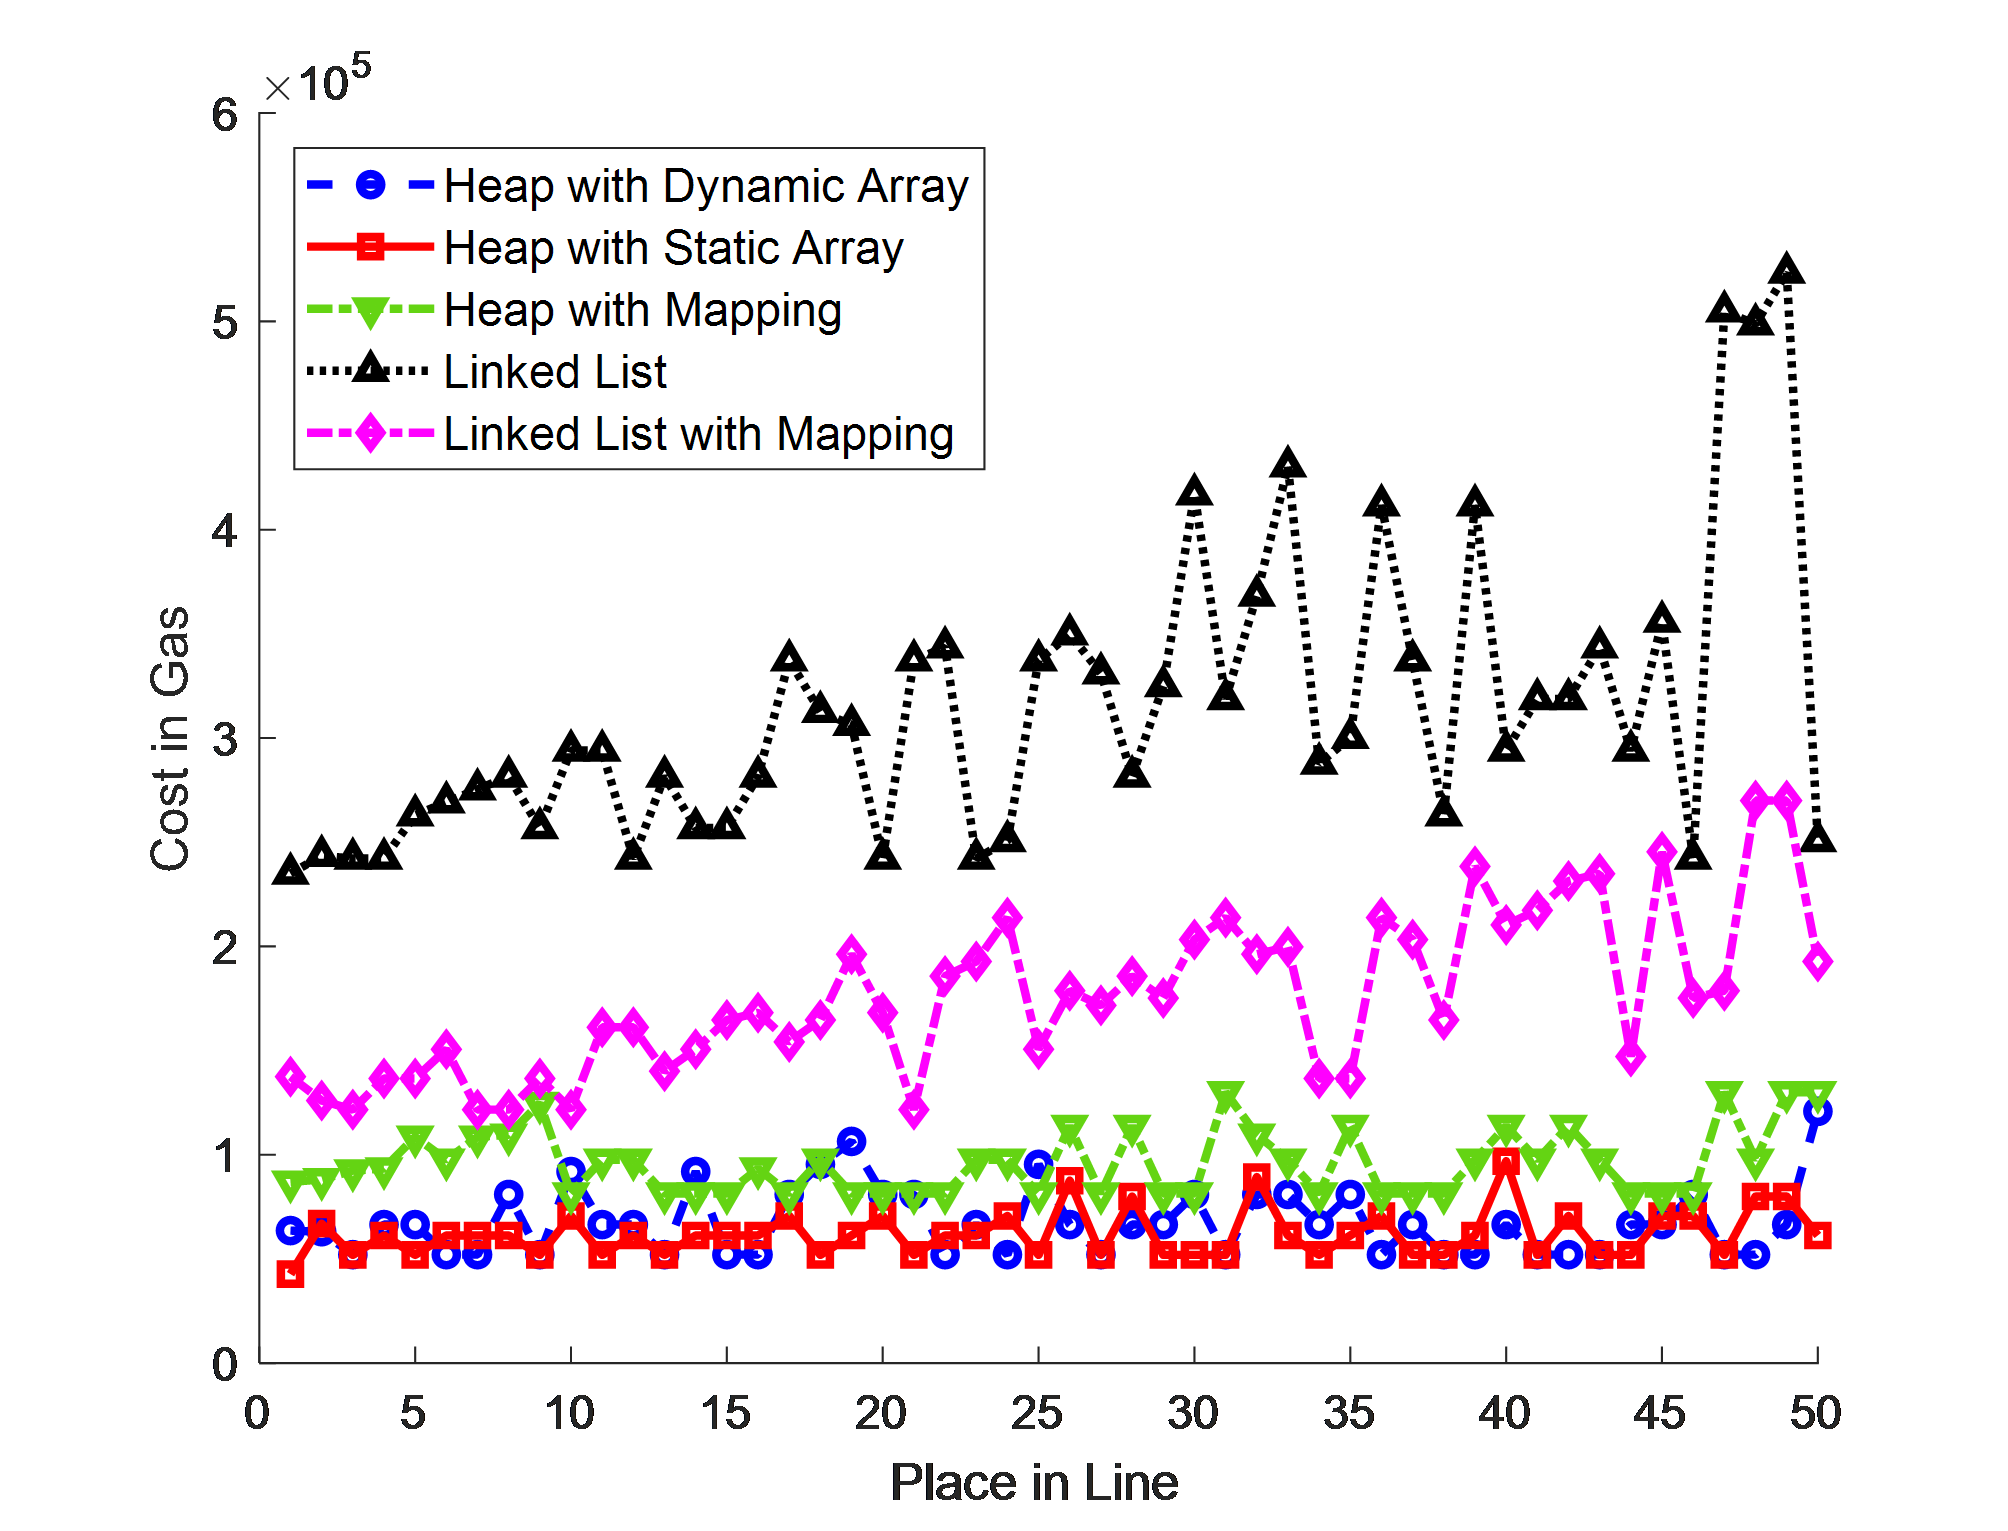
\includegraphics[width=0.5\textwidth]{fig/random_insertion3.png}
%\caption{\textblue{put the block gas limit in the chart} Gas costs for enqueuing 50 random integers into five priority queue variants. For the x-axis, a value of 9 indicates it is the 9th integer entered in the priority queue. The y-axis is the cost of enqueuing in gas.  \label{fig:random_insertion}}
%\end{figure}

% = = = = = = = = = = = = = = = = = = = = = = = = = = = = = = = = = = = = = = = =  %

%% !TEX root = ../main.tex

% = = = = = = = = = = = =Gas costs and refunds for Dequeueing 50 integers from each PQ  = = = = = = = = = = = = =  %

\begin{table}[t]
\setlength{\tabcolsep}{0.2\tabcolsep}% Shrink \tabcolsep
\centering
\begin{tabular}{|c|c|c|l|}

\multicolumn{1}{c}{} & \headrow{\footnotesize Gas Costs (\texttt{gasUsed})} & \headrow{\footnotesize Potential Refund} & \headrow{\footnotesize Full Refund?} \\ \hline

% = = = = = = = = = = = = = = = = = = = = = = = = = = = = = = = = = = = = = = = = = = = = = = = = = = = = = = = = = = = = = = = = = = = = = = %
Heap with Dynamic Array       	& 2,518,131          & 750,000     &\full                  \\ \hline
% = = = = = = = = = = = = = = = = = = = = = = = = = = = = = = = = = = = = = = = = = = = = = = = = = = = = = = = = = = = = = = = = = = = = = = %
Heap with Static Array          	& 1,385,307                             & 750,000      &\full                \\ \hline
% = = = = = = = = = = = = = = = = = = = = = = = = = = = = = = = = = = = = = = = = = = = = = = = = = = = = = = = = = = = = = = = = = = = = = = %
Heap with Mapping 			& 2,781,684                            & 1,500,000    &\full                 \\ \hline
% = = = = = = = = = = = = = = = = = = = = = = = = = = = = = = = = = = = = = = = = = = = = = = = = = = = = = = = = = = = = = = = = = = = = = = %
Linked List                     		& 557,085               	           & 1,200,000      &\full                \\ \hline
% = = = = = = = = = = = = = = = = = = = = = = = = = = = = = = = = = = = = = = = = = = = = = = = = = = = = = = = = = = = = = = = = = = = = = = %
Linked List with Mapping      	& 731,514              	     	  &  3,765,000      &\full                 \\ \hline
% = = = = = = = = = = = = = = = = = = = = = = = = = = = = = = = = = = = = = = = = = = = = = = = = = = = = = = = = = = = = = = = = = = = = = = %

\end{tabular}
\caption{The gas metrics associated with dequeuing 50 integers from five priority queue variants. For the refund, (\full) indicates the  refund was capped at the maximum amount and (\prt) means a greater refund would be possible.
\label{tab:PQUnitTests}}
\end{table}
% = = = = = = = = = = = = = = = = = = = = = = = = = = = = = = = = = = = = =  %


% = = = = = = = = = = = = = = = = = = = = = = = = = = = = = = = = = = = = = = = =  %
%  = = = = = = Table 2 (dequeue) Conversions = = = = = = %
%
%As of July 2020,  $1 gas = 56\times10^{-9} ether$\footnote{https://ethstats.net/} and 1 ether = \$238.33\footnote{https://coinmarketcap.com/}.
%
%$Transaction cost (eth) = GasUsed (unit) \times Gas Price (eth)$ 
%
%%  = = = = = = Transaction Costs in eth = = = = = = %
%
%Heap with Dynamic Array:    		$2,518,131 \times 56\times10^{-9} = 141,015,336\times 10^{-9}$
%Heap with Dynamic Array:     		$1,385,307 \times 56\times10^{-9} = 77,577,192\times 10^{-9}$
%Heap with Mapping:              		$2,781,684 \times 56\times10^{-9} = 155,774,304\times 10^{-9}$
%Linked List:						$557,085 \times 56\times10^{-9} = 	31,196,760\times 10^{-9}$
%Linked List with Mapping:			$731,514 \times 56\times10^{-9} = 	40,964,784\times 10^{-9}$
%
%%  = = = = = = Transaction Costs in USD = = = = = = %
%
%Heap with Dynamic Array:    		$141,015,336\times 10^{-9} \times 238.33 = \$33.60$
%Heap with Dynamic Array:     		$77,577,192\times 10^{-9} \times 238.33 = \$18.48$
%Heap with Mapping:              		$155,774,304\times 10^{-9} \times 238.33 = \$37.12$
%Linked List:						$31,196,760\times 10^{-9} \times 238.33 = \$7.43$
%Linked List with Mapping:			$40,964,784\times 10^{-9} \times 238.33 = \$9.76$
%
% = = = = = = = = = = = = = = = = = = = = = = = = = = = = = = = = = = = = =  %




\begin{figure}[t]
\begin{floatrow}
\ffigbox{%
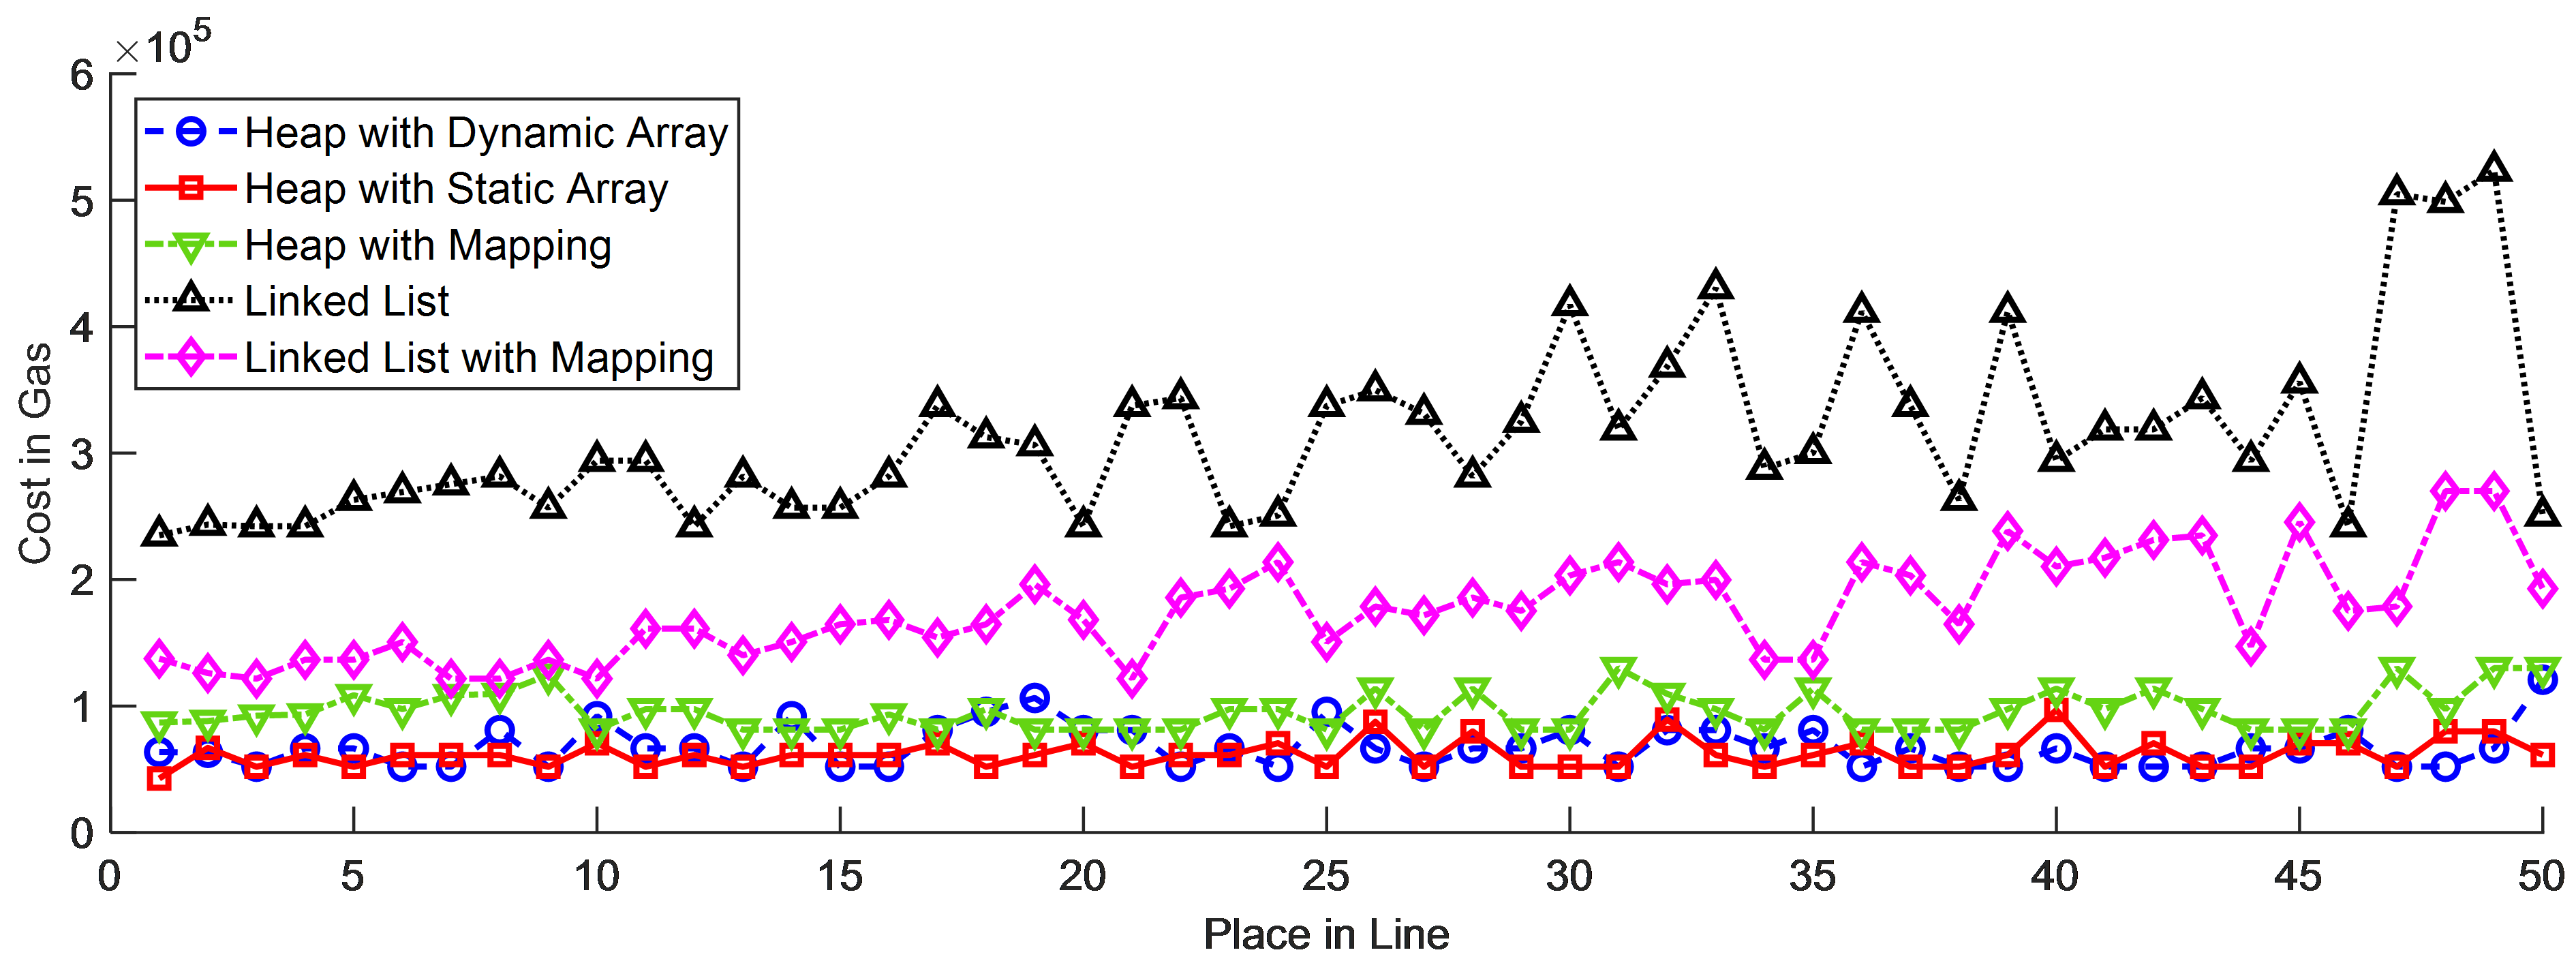
\includegraphics[width=6cm]{fig/2.png}%
}{%
  \caption{\scriptsize{Gas costs for enqueuing 50 random integers into five priority queue variants. For the x-axis, a value of 9 indicates it is the 9th integer entered in the priority queue. The y-axis is the cost of enqueuing in gas}. \label{fig:random_insertion}}%
  
}
\capbtabbox{%
\scriptsize
\begin{tabular}{|>{\centering}m{2cm} |>{\centering}m{1.15cm} |>{\centering}m{1.15cm} |>{\centering\arraybackslash}m{0.2cm}|}%{|c|c|c|c|}

\multicolumn{1}{c}{} & \headrowsidebyside{\scriptsize{\shortstack{Gas Costs \\\textit{(gwei)}}}} & \headrowsidebyside{\scriptsize{Refund \textit{(gwei)} }} & \headrowsidebyside{\scriptsize{Full Refund?}} \\ \hline

% = = = = = = = = = = = = = = = = = = = = = = = = = = = = = = = = = = = = = = = = = = = = = = = = = = = = = = = = = = = = = = = = = = = = = = %
\shortstack{Heap with\\Dynamic Array}        	& 2,518,131          & 750,000     &\full                  \\ \hline
% = = = = = = = = = = = = = = = = = = = = = = = = = = = = = = = = = = = = = = = = = = = = = = = = = = = = = = = = = = = = = = = = = = = = = = %
\shortstack{Heap with\\ Static Array}          	& 1,385,307                             & 750,000      &\full                \\ \hline
% = = = = = = = = = = = = = = = = = = = = = = = = = = = = = = = = = = = = = = = = = = = = = = = = = = = = = = = = = = = = = = = = = = = = = = %
\shortstack{Heap with\\ Mapping}  		& 2,781,684                            & 1,500,000    &\full                 \\ \hline
% = = = = = = = = = = = = = = = = = = = = = = = = = = = = = = = = = = = = = = = = = = = = = = = = = = = = = = = = = = = = = = = = = = = = = = %
Linked List                     		& 557,085               	           & 1,200,000      &\full                \\ \hline
% = = = = = = = = = = = = = = = = = = = = = = = = = = = = = = = = = = = = = = = = = = = = = = = = = = = = = = = = = = = = = = = = = = = = = = %
\shortstack{Linked List with\\ Mapping}       	& 731,514              	     	  &  3,765,000      &\full                 \\ \hline
% = = = = = = = = = = = = = = = = = = = = = = = = = = = = = = = = = = = = = = = = = = = = = = = = = = = = = = = = = = = = = = = = = = = = = = %

\end{tabular}
}{%
 \caption{\scriptsize{The gas metrics associated with dequeuing 50 integers from five priority queue variants. Full refund amount is shown but the actual refund that is applied is capped.}
\label{tab:PQUnitTests}}%
}
\end{floatrow}
\end{figure}

%\vspace{-3em}







% = = = = = = = = = = = = = = = = = = = = = = = = = = = = = = = = = = = = = = = =  %

We observe that (i) the linked list variants are materially cheaper than the heap variants at dequeuing; (ii) dequeuing in a call market must be done as a batch, whereas enqueuing is paid for one at a time by the trader submitting the order; and (iii) Ethereum will not permit more than hundreds of orders so asymptotic behaviour is not significant. For these reasons, we suggest using one of the linked list variants. As it can be seen in Figure~\ref{fig:random_insertion}, the associated cost for inserting elements into a linked list PQ is significantly greater than the linked list with mapping, as each insertion causes the creation of a new contract. Accordingly, we choose to implement the call market with the linked list with mapping which balances a moderate gas cost for insertion (\ie order submission) with one for removal (\ie closing the market and matching the orders). In Section~\ref{sec:rollups}, we implement \cm on Layer 2. There the PQ variant does not change the layer 1 gas costs and the the number of orders can be substantially increased. In this new context, we reconsider asymptotics and choose a heap (with dynamic array) to lower costs L2 gas costs across both enqueuing and dequeuing.

% = = = = = = = = = = = = = = = = = = = = = = = = = = = = = = = = = = = = = = = =  %

\subsection{Cost/Benefit of Cleaning Up After Yourself}
\label{sec:gasrefund}

% !TEX root = ../main.tex


% = = = = = = = = = = = =Gas costs and refunds for Dequeueing 50 integers from each PQ  = = = = = = = = = = = = =  %

\begin{table}[t]
\setlength{\tabcolsep}{0.1\tabcolsep}% Shrink \tabcolsep
\centering
%\scriptsize
%\begin{tabular}{|>{\centering}m{6cm} |>{\centering}m{1.5cm} |>{\centering}m{1.5cm} |>{\centering\arraybackslash}m{0.5cm}|}%{|c|c|c|c|}
\begin{tabular}{|>{\centering}m{7cm} |>{\centering}m{1.5cm} |>{\centering}m{1.5cm} |>{\centering\arraybackslash}m{0.5cm}|}%{|c|c|c|c|}

%headrows was scriptsized
\multicolumn{1}{c}{} & \headrowcleaning{Gas Used} & \headrowcleaning{Potential Refund} & \headrowcleaning{Full Refund?} \\ \hline

% = = = = = = = = = = = = = = = = = = = = = = = = = = = = = = = = = = = = = = = = = = = = = = = = = = = = = = = = = = = = = = = = = = = = = = %
% = = = = = = = = = = = = = = = = = = = = = = = = = = = = = = = = = = = = = = = = = = = = = = = = = = = = = = = = = = = = = = = = = = = = = = %
Linked List without \texttt{SELFDESTRUCT}        		& 721,370          & 0     &\prt  \\ \hline
Linked List with \texttt{SELFDESTRUCT}			& 557,085          & 1,200,000     &\full  \\ \hline
Linked List with Mapping and without \texttt{DELETE}    & 334,689          & 765,000     &\full  \\ \hline
Linked List with Mapping and \texttt{DELETE}		& 731,514          & 3,765,000     &\full  \\ \hline

% = = = = = = = = = = = = = = = = = = = = = = = = = = = = = = = = = = = = = = = = = = = = = = = = = = = = = = = = = = = = = = = = = = = = = = %
% = = = = = = = = = = = = = = = = = = = = = = = = = = = = = = = = = = = = = = = = = = = = = = = = = = = = = = = = = = = = = = = = = = = = = = %
% = = = = = = = = = = = = = = = = = = = = = = = = = = = = = = = = = = = = = = = = = = = = = = = = = = = = = = = = = = = = = = = = = = = = = = %
%caption was footnote
\end{tabular}
\caption{The gas metrics associated with dequeuing 50 integers from four linked list variants. For the refund, (\full) indicates the  refund was capped at the maximum amount and (\prt) means a greater refund would be possible.\label{tab:cleaning}}
\end{table}


%  = = = = = = Table 3 (cleaning.tex) Conversions = = = = = = %

%As of July 2020,  $1 gas = 56\times10^{-9} ether$\footnote{https://ethstats.net/} and 1 ether = \$238.33\footnote{https://coinmarketcap.com/}.
%
%$Transaction cost (eth) = GasUsed (unit) \times Gas Price (eth)$ 
%
%%  = = = = = = Transaction Costs in eth = = = = = = %
%
%Linked List w/o \texttt{SELFDESTRUCT}:     				$721,370 \times 56\times10^{-9} =  40,396,720\times 10^{-9}$ 

%Linked List with \texttt{SELFDESTRUCT}:     				$557,085 \times 56\times10^{-9} =  31,196,760\times 10^{-9}$  

%Linked List with Mapping and w/o \texttt{DELETE}: 		$334,689 \times 56\times10^{-9} =  18,742,584\times 10^{-9}$ 

%Linked List with Mapping and \texttt{DELETE}:    			$731,514 \times 56\times10^{-9} =  40,964,784\times 10^{-9}$ 

%
%%  = = = = = = Transaction Costs in USD = = = = = = %
%
%Linked List w/o \texttt{SELFDESTRUCT}:     				$40,396,720\times 10^{-9} \times 238.33 = \$9.62$

%Linked List with \texttt{SELFDESTRUCT}:     				$31,196,760\times 10^{-9}  \times 238.33 = \$7.43$

%Linked List with Mapping and w/o \texttt{DELETE}: 		$18,742,584\times 10^{-9} \times 238.33 = \$4.46$

%Linked List with Mapping and \texttt{DELETE}:    			$40,964,784\times 10^{-9}  \times 238.33 = \$9.76$

% = = = = = = = = = = = = = = = = = = = = = = = = = = = = = = = = = = = = =  %



One consequence of a linked list is that a new contract is created for every node in the list. Beyond being expensive for adding new nodes (a cost that will be bared by the trader in a call market), it also leaves a large footprint in the active Ethereum state, especially if we leave the nodes on the blockchain in perpetuity (\ie we just update the head node of the list and leave the previous head `dangling'). However in a PQ, nodes are only removed from the head of the list; thus the node contracts could be `destroyed' one by one using an extra operation, \texttt{SELFDESTRUCT}, in the \texttt{Dequeue()} function. As shown in Table~\ref{tab:cleaning}, the refund from doing this outweighs to the cost of the extra computation: gas costs are reduced from 721K to 557K.  This suggests a general principle: cleaning up after yourself will pay for itself in gas refunds. Unfortunately, this is not universally true as shown by applying the same principle to the linked list with mapping.

Dequeuing in a linked list with mapping can be implemented in two ways. The simplest approach is to process a node, update the head pointer, and leave the `removed' node's data behind in the mapping untouched (where it will never be referenced again). Alternatively, we can call \texttt{DELETE} on each mapping entry once we finish processing a trade. As it can be seen in the last two rows of Table~\ref{tab:cleaning}, leaving the data on the blockchain is cheaper than cleaning it up.

The lesson here is that gas refunds incentivize developers to clean up storage variables they will not use again, but it is highly contextual as to whether it will pay for itself. Further, the cap on the maximum refund means that refunds are not fully received for large cleanup operations (however removing the cap impacts the miners' incentives to include the transaction).  In Appendix~\ref{app:clean}, we present a second case study of the cost-benefits of clearing a mapping when it is no longer needed (including our idea to store the mapping in its own contract so it can \texttt{SELFDESTRUCT} with a single function call). The unfortunate takeaway is, again, that it is cheapest to leave the mapping in place. Cleaning up EVM state is a complicated and under-explored area of Ethereum in the research literature. For our own work, we strive to be good citizens of Ethereum and clean up to the extent that we can---thus all PQs in Table~\ref{tab:PQUnitTests} implement some cleanup.


%============= Performance =================== %

 \subsection{\cm Performance Measurements}

 % !TEX root = ../main.tex




% = = = = = = = = = = = = = = = = = = = = = = = = = = = = = = = = = = = = =  %
%Previous Table (before adding Arbitrum data):

 %= = = = = = = = = = = = = = = = = = = = = = = = = = = = = = = = = = = = =  %
\begin{table}[t]
\setlength{\tabcolsep}{0.1\tabcolsep}% Shrink \tabcolsep
\centering
\scriptsize
\begin{tabular} {|>{\centering}m{3.5cm} |>{\centering}m{0.5cm} |>{\centering}m{1.5cm} |>{\centering}m{1.8cm} |>{\centering\arraybackslash}m{1.5cm}|}
%{|c|c|c|c|c|}%{|l|r|r|r|r|}

\multicolumn{1}{c}{} & 

\headrowperformance{\scriptsize {Max Trades (w.c.)}} & 
\headrowperformance{\scriptsize {Gas Used for Max Trades }} & 
\headrowperformance{\scriptsize {Gas Used for 1000 Trades }} & 
\headrowperformance{\scriptsize{ \shortstack{Gas Used for Submission\\ (avg)}}} \\ \hline

% = = = = = = = = = = = = = = = = = = = = = = = = = = = = = = = = = = = = = = = = = = = = = = = = = = = = = = = = = = = = = = = = = = = = = = %
Heap with Dynamic Array       & 38            & 5,372,679                   	& 457,326,935      & 207,932     \\ \hline
% = = = = = = = = = = = = = = = = = = = = = = = = = = = = = = = = = = = = = = = = = = = = = = = = = = = = = = = = = = = = = = = = = = = = = = = = = = = = = = = = = %
Heap with Static Array         	& 42            & 5,247,636                  	& 333,656,805         & 197,710         \\ \hline
% = = = = = = = = = = = = = = = = = = = = = = = = = = = = = = = = = = = = = = = = = = = = = = = = = = = = = = = = = = = = = = = = = = = = = = = = = = = = = = = = = %
Heap with Mapping 		& 46           	 & 5,285,275                     & 226,499,722    & 215,040           \\ \hline
% = = = = = = = = = = = = = = = = = = = = = = = = = = = = = = = = = = = = = = = = = = = = = = = = = = = = = = = = = = = = = = = = = = = = = = = = = = = = = = = = = %
Linked List                     	& 152            & 5,495,265                     & 35,823,601         & 735,243             \\ \hline
% = = = = = = = = = = = = = = = = = = = = = = = = = = = = = = = = = = = = = = = = = = = = = = = = = = = = = = = = = = = = = = = = = = = = = = = = = = = = = = = = = %
Linked List with Mapping     	& 86             & 5,433,259                     & 62,774,170        &  547,466              \\ \hline
% = = = = = = = = = = = = = = = = = = = = = = = = = = = = = = = = = = = = = = = = = = = = = = = = = = = = = = = = = = = = = = = = = = = = = = = = = = = = = = = = = %

\end{tabular}
\caption{\footnotesize{Performance of \cm for each PQ variant. Each consumes just under the block gas limit ($\sim$11M gas) with a full refund of half of its gas.}\label{tab:worst_case_matching}}





\end{table}
% = = = = = = = = = = = = = = = = = = = = = = = = = = = = = = = = = = = = =  %





The main research question is how many orders can be processed under the Ethereum block gas limit. The choice of PQ implementation is the main influence on performance and the results are shown in Table~\ref{tab:worst_case_matching}. These numbers are for the \textit{worst-case}---when every submitted bid and ask is marketable (\ie will require fulfillment). In practice, once \texttt{closeMarket()} hits the first bid or ask that cannot be executed, it can stop processing all remaining orders. Premised on Ethereum becoming more efficient over time, we were interested in how much gas it would cost to execute 1000 pairs of orders, which is given in the third column. The fourth column indicates the cost of submitting a bid or ask --- since this cost will vary depending on how many orders are already submitted (recall Figure~\ref{fig:random_insertion}), we average the cost of 200 order submissions.

The main takeaway is that call markets appear to be limited to processing about a hundred orders per transaction and even that is at the enormous cost of monopolizing an entire Ethereum block just to close the market. Perhaps \cm can work today in some circumstances like very low liquidity tokens, or markets with high volumes and a small number of traders (\eg liquidation auctions).

% = = = = = = = = = = = = = = = = = = = = = = = = = = = = = = = = = = = = = = = = = =
% = = = = = = = = = = = = = = = = = = = = = = = = = = = = = = = = = = = = = = = = = =
% = = = = = = = = = = = = = = = = = = = = = = = = = = = = = = = = = = = = = = = = = =


\section{\cm on Arbitrum}
\label{sec:rollups}

\textit{Layer 2 (L2)} solutions~\cite{gudgeon2020sok} are a group of scaling technologies proposed to address specific drawbacks of executing transactions on Ethereum, which is considered \textit{Layer 1 (L1)}. Among these proposals, \textit{roll-ups} prioritize reducing gas costs (as opposed to other valid concerns like latency and throughput, which are secondary for \cm). We review two variants, \textit{optimistic roll-ups} and \textit{zk roll-ups}, in Appendix~\ref{app:rollup}. Briefly, in a roll-up, every transaction is stored (but not executed) on Ethereum, then executed off-chain, and the independently verifiable result is pushed back to Ethereum, with some evidence of being executed correctly. In the Appendix, we also compare \cm on Arbitrum to Loopring 3.0.

We choose to experiment with \cm on the optimistic rollup Arbitrum.\footnote{See \url{https://offchainlabs.com} for more current details than the 2018 \textit{USENIX Security} paper~\cite{kalodner2018arbitrum}.} To deploy a DApp on Arbitrum, or to execute a function on an existing Arbitrum DApp, the transaction is sent to an \textit{inbox} on L1. It is not executed on L1, it is only recorded (as calldata) in the inbox. An open network of \textit{validators} watch the inbox for new transactions. Once inbox transactions are finalized in an Ethereum block, validators will execute the transactions and assert the result of the execution to other validators on a sidechain called \textsf{ArbOS}. As the Inbox contract maintains all Arbitrum transactions, anyone can recompute the entire current state of the ArbOS and file a dispute if executions are not correctly reported on ArbOS. Disputes are adjudicated by Ethereum itself and require a small, constant amount of gas, invariant to how expensive the transaction being disputed is. When the dispute challenge period is over, the new state of ArbOS is stored as a checkpoint on Ethereum. 



% = = = = = = = = = = = = = = = = = = = = = = = = =  %
\subsection{\cm Performance Measurements on Arbitrum}
% !TEX root = ../main.tex

\begin{table}[t]
%\%setlength{\tabcolsep}{0.1\tabcolsep}% Shrink \tabcolsep
\centering
\footnotesize

\begin{tabular} {|>{\centering}m{3cm}|>{\centering}m{3cm}|>{\centering}m{3cm}|}


 \multicolumn{1}{c}{} 								&  \multicolumn{1}{c}{\textbf{Layer1  gasUsed}}										&\multicolumn{1}{c}{\textbf{Layer2 ArbGas}} 	\tabularnewline \hline
% = = = = = = = = = = = = = = = = = = = = = = = = = = = = = = = = = = = = = = = = = = = = = = = = = = = = = = = = = = = = = == = = = = = = = = = = = = = = = = = = = = = = = = = = = = = = = = = = = = = = = = = = = = = = = = = = = = = = = = = = = = = = = =  = = = %
\cm  				         		& 5,372,679              	   									& N/A							\tabularnewline \hline
% = = = = = = = = = = = = = = = = = = = = = = = = = = = = = = = = = = = = = = = = = = = = = = = = = = = = = = = = = = = = = = = = = == = = = = = = = = = = = = = = = = = = = = = = = = = = = = = = = = = = = = = = = = = = = = = = = = = = = = = = = = = = = = = = = = %
\cm on Arbitrum 				      & 6,569 													& 508,250								\tabularnewline \hline
% = = = = = = = = = = = = = = = = = = = = = = = = = = = = = = = = = = = = = = = = = = = = = = = = = = = = = = = = = = = = = = = = = == = = = = = = = = = = = = = = = = = = = = = = = = = = = = = = = = = = = = = = = = = = = = = = = = = = = = = = = = = = = = = = = = %

\end{tabular}
\caption{L1 vs L2.\label{tab:arbitrum_performance}}

\end{table}
% = = = = = = = = = = = = = = = = = = = = = = = = = = = = = = = = = = = = =  %

%txs from Arbitrum explorer:

%1- Heap with Dynamic Array : https://explorer.arbitrum.io/#/tx/0x36587f3126d6bb3a514810125be1c4adbdae94a297498406d855c0dc7ef19b05
%2- Heap with Static Array : https://explorer.arbitrum.io/#/tx/0x6be08b5b3961f0872465f9f037a20f256e23d2a78ba9f2a5537843d30ea64dd3
%3- Heap with Mapping : https://explorer.arbitrum.io/#/tx/0x54bbda54c8f720fecc5c9573e02729d8834540ab6f8fb1102a499abab71d31b0
%4- Linked List  : https://explorer.arbitrum.io/#/tx/0xb6625f4f3a2f5084b637ea79448943e24056a9693a4409de05bb3c48be42839d
%5- Linked List with Mapping : https://explorer.arbitrum.io/#/tx/0x2b3d9ff73cb992a911a047f3ade89ba05ae4eade2a5869bf610b6fd0dc091054



% = = = = = = = = = = = = = =The Entire Performance Table with Arbitrum = = = = = = = = = = = = = = = = =  %
 
%\begin{table*}[t]
%%\%setlength{\tabcolsep}{0.1\tabcolsep}% Shrink \tabcolsep
%\centering
%\begin{tabular} {|l|r|r|r|r|r|r|r|}
%
%
%\multicolumn{1}{c}{} & 
%
%
%
%\headrow{\footnotesize \shortstack{Max trades \\ (w.c.)}} & 
%\headrow{\footnotesize \shortstack{L1 Gas for \\ max trades}} & 
%\headrow{\footnotesize \shortstack{Gas for \\1000 trades}} & 
%\headrow{\footnotesize Gas for order (avg)} &
%
%\headrow{\footnotesize \shortstack{L1 Gas for \\ max trades}} &
%\headrow{\footnotesize \shortstack{L2 ArbGas \\for \\max trades}} &
%\headrow{\footnotesize Size}  \\ \hline
%
%% = = = = = = = = = = = = = = = = = = = = = = = = = = = = = = = = = = = = = = = = = = = = = = = = = = = = = = = = = = = = = = = = = = = = = = = = = = = = = = = = = = = = = = = = = = = = = = = = = = = = = = = = = = = = = = = = = = = = = = = = = = = = = = = = = = %
%\multicolumn{1}{|c|}{} &                                                            \multicolumn{4}{c|}{\textbf{Ethereum}}&                                                                                                            \multicolumn{3}{c|}{\textbf{Arbitrum}} 														\\ \hline
%% = = = = = = = = = = = = = = = = = = = = = = = = = = = = = = = = = = = = = = = = = = = = = = = = = = = = = = = = = = = = = == = = = = = = = = = = = = = = = = = = = = = = = = = = = = = = = = = = = = = = = = = = = = = = = = = = = = = = = = = = = = = = = =  = = = %
%Heap with Dynamic Array      				& 38            		& 5,372,679                   	& 457,326,935      	& 207,932     						& 1,544					& 46,705,693					& 103								\\ \hline
%% = = = = = = = = = = = = = = = = = = = = = = = = = = = = = = = = = = = = = = = = = = = = = = = = = = = = = = = = = = = = = = = = = == = = = = = = = = = = = = = = = = = = = = = = = = = = = = = = = = = = = = = = = = = = = = = = = = = = = = = = = = = = = = = = = = %
%Heap with Static Array       					& 42            		& 5,247,636                  	& 333,656,805        	 & 197,710        					& 1,402					& 46,311,418					& 103									 \\ \hline
%% = = = = = = = = = = = = = = = = = = = = = = = = = = = = = = = = = = = = = = = = = = = = = = = = = = = = = = = = = = = = = = = = = = = = = = = = = = = = = = = = = = = = = = = = = = = = = = = = = = = = = = = = = = = = = = = = = = = = = = = = = = = = = = = = = = = %
%Heap with Mapping 						& 46           	 	& 5,285,275                     	& 226,499,722    		& 215,040           					& 1,339					& 50,395,993					& 103									\\ \hline
%% = = = = = = = = = = = = = = = = = = = = = = = = = = = = = = = = = = = = = = = = = = = = = = = = = = = = = = = = = = = = = = = = = = = = = = = = = = = = = = = = = = = = = = = = = = = = = = = = = = = = = = = = = = = = = = = = = = = = = = = = = = = = = = = = = = = %
%Linked List                     					& 152            		& 5,495,265                     	& 35,823,601         	& 735,243             				& 1,325					& 99,514,286					& 103									\\ \hline
%% = = = = = = = = = = = = = = = = = = = = = = = = = = = = = = = = = = = = = = = = = = = = = = = = = = = = = = = = = = = = = = = = = = = = = = = = = = = = = = = = = = = = = = = = = = = = = = = = = = = = = = = = = = = = = = = = = = = = = = = = = = = = = = = = = = = %
%Linked List with Mapping     				& 86             		& 5,433,259                     	& 62,774,170        	&  547,466              				& 1,319					& 58,035,156					& 103									\\ \hline
%% = = = = = = = = = = = = = = = = = = = = = = = = = = = = = = = = = = = = = = = = = = = = = = = = = = = = = = = = = = = = = = = = = = = = = = = = = = = = = = = = = = = = = = = = = = = = = = = = = = = = = = = = = = = = = = = = = = = = = = = = = = = = = = = = = = = %
%
%\end{tabular}
%\caption{Performance of \cm for each PQ variant. Each consumes just under the block gas limit ($\sim$11M gas) with a full refund of half of its gas \textblue{update the caption now that we have the Arbitrum data}.\label{tab:arbitrum_performance}}
%
%\end{table*}
%% = = = = = = = = = = = = = = = = = = = = = = = = = = = = = = = = = = = = =  %






\textit{Testing Platforms.} We implement \cm using the Arbitrum Rollup chain hosted on the Rinkeby testnet.  It is visible and can be interacted with here: \href{https://rinkeby-explorer.arbitrum.io/address/0x0aa5449a9f7fa34a81ce1dc720563938a27e8b03}{[Arbitrum Explorer]}. To call functions on \cm, traders can (i) send transactions directly to the \href{https://rinkeby.etherscan.io/address/0x578BAde599406A8fE3d24Fd7f7211c0911F5B29e}{Inbox contract}, or (ii) use a relay server (called a \textit{Sequencer}) provided by the Arbitrum. The sequencer will group, order, and send all pending transactions together as a single Rinkeby transaction to the inbox (and pays the gas).

In our \cm variant on Arbitrum, the validators do all computations (both enqueuing and dequeuing) so we choose to use a heap with dynamic array for our priority queue, which balances the expense of both operations. Heaps are 32\% more efficient than linked lists for submitting orders and 29\% less efficient for closing. Recall that without a roll-up, such a priority queue can only match 38 pairs at a cost of 5,372,679 gas. Table~\ref{tab:arbitrum_performance} shows that 38 pairs cost only 6,569 in L1 gas (a 99.88\% savings). This is the cost of submitting the \texttt{closeMarket()} transaction to the inbox to be recorded, which is 103 bytes of calldata. Most importantly, \texttt{closeMarket()} always costs 6,569 even as the number of trades increase from 38 pairs. Of course, as the number of trades increase, the work for the validators on L2 increases, as measured in ArbGas. The price of ArbGas in Gwei is not well-established but is anticipated to be relatively cheap. Finally, for traders submitting an order, the L1 cost is reduced from 207,932 to 6,917.

Running \cm on Arbitrum has one large caveat. If the ERC20 tokens being traded are not issued on ArbOS, which is nearly always the case today, they first need to be \textit{bridged} onto ArbOS, as does the ETH. Traders send ETH or tokens to Arbitrum's bridge contracts which create the equivalent amount at the same address on L2. Withdrawals work the same way in reverse, but are only final on Layer 1 after a dispute challenge period (currently 1 hour).\footnote{Layer 1 users might accept assets before they are finalized as they can determine their eventual emergence on Layer 1 is indisputable (\textit{eventual finality}).}

% = = = = = = = = = = = = = = = = = = = = = = = = =  %

\section{Design Alternatives and Extensions}

\cm is designed as a base class that can be extended and customized. Here, we evaluate potential modifications.

\begin{figure}[t]
\centering
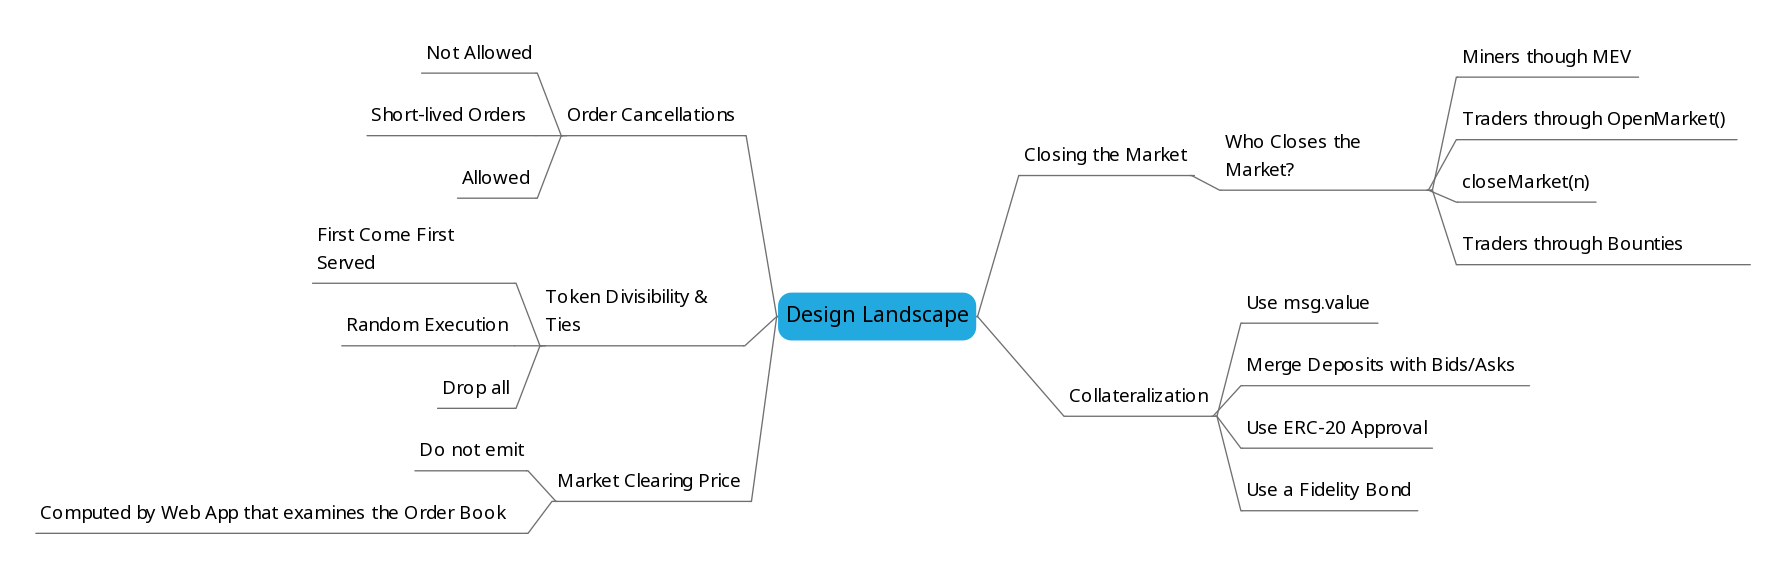
\includegraphics[width=1\textwidth]{fig/MindMapDraft3.png}
\caption{\footnotesize{Mind Map Draft}  \label{fig:rmindmap}}
\end{figure}
% = = = = = = = = = = = = = = = = = = = = = = = = =  %

\subsection{Token Divisibility and Ties}

When executing trades, if the volume of the current best bid does not match the best ask, the larger order is partially filled and the remaining volume is considered against the next best order. A common trading rule (that does resist front-running) is to fill ties in proportion to their volume (\ie \textit{pro rata} allocation)\footnote{If Alice and Bob bid the same price for 100 tokens and 20 tokens respectively, and there are only 60 tokens left in marketable asks, Alice receives 50 and Bob 10.}, however this approach does not always work. Consider the following corner case: 3 equally priced bids of 1 non-divisible token and 1 ask at the same price. There is no good option: (1) the bids could all be dropped, (2) the bids could be prioritized based on time, or (3) the bid could be randomly chosen (\cf Libra~\cite{mavroudis2019libra}).

\paragraph{Evaluation.} We avoid (1) which is fair but not market efficient. We note the conditions under which pro rata allocation fails (\ie non-divisible assets, an exact tie on price, and part of the final allocation) are improbable. In \cm, tokens are assumed to be divisible but we otherwise default to (2). This means insertion front-running attacks are possible for this corner case. However if these attacks proved to be a problem in practice, (3) is a better solution with one main drawback: on-chain sources of `randomness' are generally deterministic and manipulatable by miners~\cite{bonneau2015random,buenz2017proofs}, countermeasures can take a few blocks to select~\cite{boneh2018verifiable}. 

% = = = = = = = = = = = = = = = = = = = = = = = = =  %

\subsection{Order Cancellations}
\label{sec:cancel}

\cm does not support order cancellations. We intend to open and close markets quickly (on the order of blocks), so orders are relatively short-lived.

\paragraph{Evaluation.} Support for cancellation opens the market to new front-running issues where other traders (or miners) can displace cancellations until after the market closes. However, one benefit of a call market is that beating a cancellation with a new order has no effect, assuming the cancellation is run any time before the market closes. Also, cancellations have a performance impact. Cancelled orders can be removed from the underlying data structure or accumulated in a list that is cross-checked when closing the market. Removing orders requires a more verbose structure than a priority queue (\eg a self-balancing binary search tree instead of a heap; or methods to traverse a linked list rather than only pulling from the head). While client software could help point out where the order is in the data structure, the order book can change between submitting the cancellation request and running the method. %A linked list with mapping that returns the key for each submitted order seems to be the most tenable data structure.

% = = = = = = = = = = = = = = = = = = = = = = = = =  %

\subsection{Market Clearing Price}

% JC: Not part of design landscape, find a new home for it

Call markets are heralded for fair price discovery. This is why many exchanges use a call market at the end of the day to determine the closing price of an asset, which is an important price both optically (it is well-published) and operationally (many derivatives settle based on the closing price). We purposely do not compute a `market clearing price' with \cm because miners can easily manipulate the price (\ie include a single wash trade at the price they want fixed), although they forgo profit for doing so. This is not merely hypothetical---Uniswap (the prominent quote-drive, on-chain exchange) prices have been manipulated to exploit other DeFi applications relying on them. Countermeasures to protect Uniswap price integrity could also apply to \cm: (1) taking a rolling median of prices over time, and (2) using it alongside other sources for the same price and forming a consensus. While \cm does not emit a market clearing price, it can be computed by a web application examining the order book at market close.

% = = = = = = = = = = = = = = = = = = = = = = = = =  %

\subsection{Scheduling Events}

\cm is a one-shot market. However it can be extended to reopen with a clean order book after \texttt{closeMarket()} is run. Modifiers can enforce when the market operates openly (collecting orders) and when close can be run. In the Princeton paper~\cite{clark2014decentralizing}, the call market is envisioned to run as an alt-coin, where orders accumulate within a block and a miner closes the market as part of the logic of producing a new block (\ie within the same portion of code as computing their coinbase transaction in Bitcoin or \texttt{gasUsed} in Ethereum).

If the call market runs as a DApp on Ethereum, it seems difficult to open and close the market on every block. Someone needs to call the \texttt{closeMarket()} for every block (we return to who this is later), but the market will only work as intended if miners execute this function after every \texttt{submitBid()} and \texttt{submitAsk()} invocation. Since price improvements are paid to the miners, the miner is actually incentivized to run \texttt{closeMarket()} last to make the most profit. This pattern is called miner extractable value (MEV)~\cite{daian2019flash} and is usually considered in the context of attacks. However in our case, MEV is a feature. Efficient algorithms for miners to automatically find MEV opportunities is an open research problem.


A close alternative is to allow markets to open and close on different blocks. In this alternative, the \texttt{closeMarket()} function calls \texttt{openMarket()} as a subroutine and sets two modifiers: orders are only accepted in the block immediately after the current block (\ie the block that executes the \texttt{closeMarket()}) and \texttt{closeMarket()} cannot be run again until two blocks after the current block.

The final issue is who invokes \texttt{closeMarket()} every other block? There are two issues here: the issue of scheduling the function call and the issue of paying for it. For scheduling the function call, we can do one of the following: rely on market participants, who are eager to trade, to reopen the market, offer a bounty to reopen the market, or use an external service like Ethereum Alarm Clock (which creates a regulatory hook).\footnote{\url{https://ethereum-alarm-clock-service.readthedocs.io/}} Next, we consider the second issue of who pays to close the market.

% = = = = = = = = = = = = = = = = = = = = = = = = =  %

\subsection{Who Pays to Close/Reopen the Market?}
\label{sec:close}

As miners are paid all price improvements in the market, it is possible that a miner might run \texttt{closeMarket()} and it would pay for itself. However, we consider two other scenarios that do not assume miners can automatically find MEV opportunities. One solution requires a modified closing function, \texttt{closeMarket(n)}, that only processes $n$ orders at a time until the order book is empty (this is sensible design in any case to safeguard against the order book from locking up because the number of orders exceeds the gas limit to process them).  Once the time window for submitting orders has past, a new market is created (without settling the previous market). Every order submission on the new market also requires to run, say, \texttt{closeMarket(10)} on the older market, thus progressively closing the previous market while accepting orders to the new market.

The second solution is to levy a carefully computed fee against the traders for every new order they submit. These fees are accumulated by the DApp to use as a bounty. When the time window for the open market elapses, the user who calls the \texttt{closeMarket()} function receives the bounty.

\paragraph{Evaluation.} The first solution pattern has two issues: first, amortizing the cost of closing the market amongst the early traders of the new market is an added incentive to not submit orders early to the market; the second issue is if not enough traders submit orders in the new market, the old market never closes (resulting in a backlog of old markets waiting to close). The second solution is better, although not perfect: \texttt{closeMarket()} cost does not follow a tight linear increase with the number of orders, and gas prices vary over time which could render the bounty insufficient for offsetting the \texttt{closeMarket()} cost. However, an interested third party (such as the token issuer for a given market) might occasionally bailout the market when it halts on \texttt{closeMarket()} to facilitate further trading. If the DApp can pay for its own functions, an interested party can also arrange for a commercial service (\eg any.sender\footnote{\url{https://github.com/PISAresearch/docs.any.sender}}) to relay the \texttt{closeMarket()} function call on Ethereum (an approach called \textit{meta-transactions}) which introduces another regulatory hook.

% = = = = = = = = = = = = = = = = = = = = = = = = =  %

\subsection{Collateralization Options}

In \cm, both the tokens and ETH that a trader wants to potentially use in the order book are pre-loaded into the contract. Consider Alice, who holds a token and decides she wants to trade it for ETH. In this model, she must first transfer the tokens to the contract and then submit an ask order. If she does this within the same block, there is a chance that a miner will execute the ask before the transfer and the ask will revert. If she waits for confirmation, this introduces a delay. This delay seems reasonable but we point out a few options it could be addressed:

\begin{enumerate}

\item \textbf{Use \texttt{msg.value}.} For the ETH side of a trade (\ie for bids), ETH could be sent with the function call to \texttt{submitBid()} to remove the need for    \texttt{depositEther()}. This works for markets that trade ERC20 tokens for ETH, but would not work for ERC20 to ERC20 exchanges.

\item \textbf{Merge Deposits with Bids/Asks.} \cm could have an additional function that atomically runs the functionality of \texttt{depositToken()} followed by the functionality of \texttt{submitAsk()}. This removes the chance that the deposit and order submission are ordered incorrectly.

\item \textbf{Use ERC20 Approval.} Instead of \cm taking custody of the tokens, the token holder could simply approve \cm to transfer tokens on her behalf. If \cm is coded securely, it is unconcerning to allow the approval to stand long-term and the trader never has to lock up their tokens in the DApp. The issue is that there is no guarantee that the tokens are actually available when the market closes (\ie Alice can approve a DApp to spend 100 tokens even if she only has 5 tokens or no tokens). In this case, \cm would optimistically try to transfer the tokens and if it fails, move onto the next order. This also gives Alice an indirect way to cancel an order, by removing the tokens backing the order---this could be a feature or it could be considered an abuse.

\item \textbf{Use a Fidelity Bond.} Traders could post some number of tokens as a fidelity bond, and be allowed to submit orders up to 100x this value using approve. If a trade fails because the pledged tokens are not available, the fidelity bond is slashed as punishment. This allows traders to side-step time-consuming transfers to and from \cm while still incentivizing them to ensure that submitted orders can actually be executed. The trade-off  is that \cm needs to update balances with external calls to the ERC20 contract instead of simply updating its internal ledger.

\end{enumerate}




% = = = = = = = = = = = = = = = = = = = = = = = = = = = = = = = = = = = = = = = = = =

\section{Front-running Evaluation} 
\label{sec:front}

% !TEX root = ../main.tex




\begin{table*}[t]

\centering
\tiny
%\resizebox{1.7\columnwidth}{!}{

\begin{tabular}{|c|c|c|c|c|c|c|c|c|c|c|c|c|}

\multicolumn{1}{c}{} &
\multicolumn{1}{c}{} &
\multicolumn{1}{c}{} &
\headrowfrontTwo{\shortstack{Centralized Continuous\\ Market (Coinbase)}} &
\headrowfrontTwo{\shortstack{Partially Off-chain Continuous\\ Market (EtherDelta)}} & 
\headrowfrontTwo{\shortstack{Partially Off-chain Continuous \\Market w/ Roll-up (Loopring)}} & 
\headrowfrontTwo{\shortstack{On-chain Continuous \\Market (OasisDex)}}  &
\headrowfrontTwo{\shortstack{On-chain Dark \\Continuous Market (TEX)}} &
\headrowfrontTwo{\shortstack{On-chain Automated \\Market Maker (Uniswap)}}  & 
\headrowfrontTwo{\shortstack{On-chain Call Market \\w/ Price Improvement}} &
\headrowfrontTwo{\shortstack{On-chain Call Market (\cm)}}  & 
\headrowfrontTwo{\shortstack{On-chain Call Market  \\w/ Roll-up (\cm variant)}}  &
\headrowfrontTwo{\shortstack{On-chain Dark \\Call Market (Galal \etal)}}
\\

%\hhline{-----------}
\hline
% = = = = = = = = = = = = = = = = = = = = = = = = = = = = = = = = = = = = = = = = = = = = = = = = = = = = = = = = = = = = = = = = = = = = = = = = = = = = = = = = = = = = = = = = = = = = = = = = = = = = = = = = = = = = = = = = = = = = = = = = = = = = = = = = = = = = = = = = = = = == = = = = = = = = = = = = = = = = = = = = = = = = = = = = = = = = = = = = %								 											
%\parbox[t]{1mm}{\multirow{10}{*}{\rotatebox[origin=c]{90}{Attack Example}}} 	&&&&&&&&&&&														\\ \hline		
	     
% = = = = = = = = = = = = = = = = = = = = = = = = = = = = = = = = = = = = = = = = = = = = = = = = = = = = = = = = = = = = = = = = = = = = = = = = = = = = = = = = = = = = = = = = = = = = = = = = = = = = = = = = = = = = = = = = = = = = = = = = = = = = = = = = = = = = = = = = = = = == = = = = = = = = = = = = = = = = = = = = = = = = = = = = = = = = = = = = %								 											
	     
%	     
%	     & \multicolumn{2}{c?{1mm}}{Classification}             																											&\multicolumn{1}{c|}{LOB}		&\multicolumn{1}{c|}{LOB}		&\multicolumn{1}{c|}{LOB}		&\multicolumn{1}{c|}{LOB}		&\multicolumn{1}{c|}{LOB}		&\multicolumn{1}{c|}{AMM}		&\multicolumn{1}{c|}{CM}		&\multicolumn{1}{c|}{CM}	&\multicolumn{1}{c|}{CM}								  										&\multicolumn{1}{c|}{CM}	 \\ \hhline{~------------}                 

% = = = = = = = = = = = = = = = = = = = = = = = = = = = = = = = = = = = = = = = = = = = = = = = = = = = = = = = = = = = = = = = = = = = = = = = = = = = = = = = = = = = = = = = = = = = = = = = = = = = = = = = = = = = = = = = = = = = = = = = = = = = = = = = = = = = = = = = = = = = == = = = = = = = = = = = = = = = = = = = = = = = = = = = = = = = = = = = = %								 											

\multicolumn{3}{|c?{1mm}}{\makecell{Who is Mallory? \\ \underline{A}uthority,  \underline{T}rader, \underline{M}iner, \underline{S}equencer	}}   	&A&A,T,M&A,T,M,S&T,M&T,M&T,M&T,M&T,M&T,M,S	&T,M	 \\ \cmidrule[1mm]{1-13}

% = = = = = = = = = = = = = = = = = = = = = = = = = = = = = = = = = = = = = = = = = = = = = = = = = = = = = = = = = = = = = = = = = = = = = = = = = = = = = = = = = = = = = = = = = = = = = = = = = = = = = = = = = = = = = = = = = = = = = = = = = = = = = = = = = = = = = = = = = = = == = = = = = = = = = = = = = = = = = = = = = = = = = = = = = = = = = = = = %								 											

\multirow{17}{*}{\rotatebox[origin=c]{90}{\textbf{Attack Example}}}		&\multicolumn{1}{c|}{\makecell{Mallory (\textit{maker}) squeezes in a\\ transaction before Alice's  (\textit{taker})  order}}  						&\multicolumn{1}{c?{1mm}}{Ins.}		&\empt	&\empt &\empt &\empt &\full &\empt &\full &\full  &\full &\full		\\ \hhline{~------------}					 					
% = = = = = = = = = = = = = = = = = = = = = = = = = = = = = = = = = = = = = = = = = = = = = = = = = = = = = = = = = = = = = = = = = = = = = = = = = = = = = = = = = = = = = = = = = = = = = = = = = = = = = = = = = = = = = = = = = = = = = = = = = = = = = = = = = = = = = = = = = = = == = = = = = = = = = = = = = = = = = = = = = = = = = = = = = = = = = = = = %								 											
								 											
&\multicolumn{1}{c|}{\makecell{Mallory (\textit{taker}) squeezes in a \\transaction before Bob's (\textit{taker 2})}   }	  								&\multicolumn{1}{c?{1mm}}{  Disp.}				&\empt &\empt &\empt &\empt &\full &\empt &\full &\full &\full	&\full		\\ \hhline{~------------}	
% = = = = = = = = = = = = = = = = = = = = = = = = = = = = = = = = = = = = = = = = = = = = = = = = = = = = = = = = = = = = = = = = = = = = = = = = = = = = = = = = = = = = = = = = = = = = = = = = = = = = = = = = = = = = = = = = = = = = = = = = = = = = = = = = = = = = = = = = = = = == = = = = = = = = = = = = = = = = = = = = = = = = = = = = = = = = = = = = %

&\multicolumn{1}{c|}{\makecell{Mallory (\textit{maker 1}) suppresses a better \\ incoming order from Alice (\textit{maker 2}) \\ until Mallory's order is executed}}																&\multicolumn{1}{c?{1mm}}{Supp.} 				&\empt &\empt &\empt &\full &\full &\full &\prt &\prt &\prt &\prt	\\ 	\hhline{~------------}				 											
% = = = = = = = = = = = = = = = = = = = = = = = = = = = = = = = = = = = = = = = = = = = = = = = = = = = = = = = = = = = = = = = = = = = = = = = = = = = = = = = = = = = = = = = = = = = = = = = = = = = = = = = = = = = = = = = = = = = = = = = = = = = = = = = = = = = = = = = = = = = == = = = = = = = = = = = = = = = = = = = = = = = = = = = = = = = = = = = = %

&\multicolumn{1}{c|}{\makecell{A hybrid attack based on the above \\ (\eg sandwich attacks, scalping)}}																		&\multicolumn{1}{c?{1mm}}{I/S/D}																		&\empt &\empt &\empt &\empt &\full &\empt &\empt &\full &\full	&\full												\\ 	\hhline{~------------}
% = = = = = = = = = = = = = = = = = = = = = = = = = = = = = = = = = = = = = = = = = = = = = = = = = = = = = = = = = = = = = = = = = = = = = = = = = = = = = = = = = = = = = = = = = = = = = = = = = = = = = = = = = = = = = = = = = = = = = = = = = = = = = = = = = = = = = = = = = = = == = = = = = = = = = = = = = = = = = = = = = = = = = = = = = = = = = = = = %

&\multicolumn{1}{c|}{\makecell{Mallory suspends the market \\for a period of time}}																										&\multicolumn{1}{c?{1mm}}{Supp.}    				&\empt  &\empt  &\empt  &\prt  &\prt  &\prt  &\prt  & \prt &\prt &\prt 	\\ 	\hhline{~------------}
% = = = = = = = = = = = = = = = = = = = = = = = = = = = = = = = = = = = = = = = = = = = = = = = = = = = = = = = = = = = = = = = = = = = = = = = = = = = = = = = = = = = = = = = = = = = = = = = = = = = = = = = = = = = = = = = = = = = = = = = = = = = = = = = = = = = = = = = = = = = == = = = = = = = = = = = = = = = = = = = = = = = = = = = = = = = = = = = = %

&\multicolumn{1}{c|}{\makecell{Spoofing: Mallory (\textit{maker}) puts an \\ order as bait, sees Alice (\textit{taker}) \\ tries to execute it, and cancels it first}}													&\multicolumn{1}{c?{1mm}}{S\&D} 				&\empt &\empt &\empt &\empt &\full &\empt &\full &\full &\full &\full \\ 	\hhline{~------------}
% = = = = = = = = = = = = = = = = = = = = = = = = = = = = = = = = = = = = = = = = = = = = = = = = = = = = = = = = = = = = = = = = = = = = = = = = = = = = = = = = = = = = = = = = = = = = = = = = = = = = = = = = = = = = = = = = = = = = = = = = = = = = = = = = = = = = = = = = = = = == = = = = = = = = = = = = = = = = = = = = = = = = = = = = = = = = = = = = %

&\multicolumn{1}{c|}{\makecell{Cancellation Griefing: Alice (\textit{maker}) \\ cancels an order and Mallory \\ (\textit{taker}) fulfills it first}}													&\multicolumn{1}{c?{1mm}}{Disp.} 							&\empt &\empt &\empt &\empt &\full &\empt &\full & \full &\full	&\full \\ 	\hline
% = = = = = = = = = = = = = = = = = = = = = = = = = = = = = = = = = = = = = = = = = = = = = = = = = = = = = = = = = = = = = = = = = = = = = = = = = = = = = = = = = = = = = = = = = = = = = = = = = = = = = = = = = = = = = = = = = = = = = = = = = = = = = = = = = = = = = = = = = = = == = = = = = = = = = = = = = = = = = = = = = = = = = = = = = = = = = = = = %



\end{tabular}

%} %end resizebox

\caption{\footnotesize{An evaluation of front-running attacks (rows) for different types of order books (columns). Front-running attacks are in three categories: \underline{Ins}ertion, \underline{disp}lacement, and \underline{supp}ression. A full dot (\tinyfull) means the front-running attack is mitigated or not applicable to the order book type, a partial mitigation (\tinyprt) is awarded when the front-running attack is possible but expensive, and we give no award (\tinyempt) if the attack is feasible}. 
\label{tab:front}}
\end{table*}







As we illustrate in Table~\ref{tab:front}, call markets have a unique profile of resilience against \emph{front-running attacks}~\cite{clark2014decentralizing,eskandari2019sok,daian2019flash} that differs somewhat from continuous-time markets and automated market makers. Traders are sometimes distinguished as \emph{makers} (adds orders to a market) and \emph{takers} (trades against a pre-existing, unexecuted orders). A continuous market has both. All traders using an automated market maker are takers, while the investors who provide tokens to the AMM (liquidity providers) are makers. Under our definition, a call market only has makers: the only way to have a trade executed is to submit an order. The front-running attacks in Table~\ref{tab:front} are sub-categorized, using a recent SoK~\cite{eskandari2019sok}, as being \emph{Insertion}, \emph{Displacement}, and \emph{Suppression}. To explain the difference, we will illustrate the first three attacks in the table.

In an \emph{insertion attack}, Mallory learns of a transaction from Alice. Consider Alice submitting a bid order for 100 tokens at any price (market order). Mallory decides to add new ask orders to the book (limit orders) at the maximum price reachable by Alice's order given the rest of the asks in the book. Mallory must arrange for her orders to be added before Alice's transaction and then arrange for Alice's transaction to be the next (relevant) transaction to run (\eg before competing asks from other traders are added).

In a centralized exchange, Mallory would collude with the \emph{authority} running the exchange to conduct this attack. On-chain, Mallory could be a fast \emph{trader} who sees Alice's transaction in the mempool and adds her transaction with a higher gas fee to bribe miners to execute hers first (insertion is probabilist and not guaranteed). Finally, Mallory could be the \emph{miner} of the block that includes Alice's transaction allowing her to insert with high fidelity. Roll-ups use \emph{sequencers} discussed in Section~\ref{sec:frontarb}.

A \emph{displacement attack} is like an insertion attack, except Mallory does not care what happens to Alice's original transaction---she only cares about being first. If Mallory sees Alice trying to execute a trade at a good price, she could try to beat Alice and execute the trade first. Mallory is indifferent to whether Alice can then execute her trade or not. The analysis of both insertion and suppression attacks are similar.  Call markets mitigate these basic insertion and displacement attacks because they do not have any time priority (e.g., if you were to shuffle the order of all orders submitted within the same call, the outcome would be exactly the same). A different way to mitigate these attacks is to seal orders with confidentiality (a \textit{dark} market).

In a \emph{suppression attack}, Mallory floods the network with transactions until a trader executes her order. Such selective denial of service is possible by an off-chain operator. With on-chain continuous markets, it is not possible to suppress Alice's transaction while also letting through a transaction from a taker---suppression applies to all Ethereum transactions or none. A call market is uniquely vulnerable because it eventually times out (which does not require an on-chain transaction) and new orders cannot be added. We still award a call market partial mitigation since suppression attacks are expensive (\cf Fomo3D attack~\cite{eskandari2019sok}). If the aim of suppression is a temporary denial of service (captured by attack 5 in the table), then all on-chain markets are vulnerable to this expensive attack.

Some attacks combine more than one insertion, displacement, and/or suppression attacks. AMMs are vulnerable to a double insertion called a sandwich attack~\cite{ZQFLG21} which bookends a victim's trade with the front-runner's trades (plus additional variants). In a traditional call market, a market clearing price is chosen and all trades are executed at this price. All bids made at a higher price will receive the assets for the lower clearing price (and conversely for lower ask prices): this is called a \textit{price improvement} and it allows traders to submit at their best price. A hybrid front-running attack allows Mallory to extract any price improvements. Consider the case where Alice's ask crosses Bob's bid with a material price improvement. Mallory inserts a bid at Alice's price, suppresses Bob's bid until the next call, and places an ask at Bob's price. She buys and then immediately sells the asset and nets the price improvement as arbitrage. To mitigate this in \cm, all price improvements are given to the miner (using \texttt{block.coinbase.transfer()}). This does not actively hurt traders---they always receive the same price that they quote in their orders---and it removes any incentive for miners to front-run these profits.

Other front-running attacks use order cancellations (see Section~\ref{sec:cancel}) which \cm mitigates by running short-lived markets with no cancellations.

There are two main takeaways from Table~\ref{tab:front}. Call markets provide strong resilience to front-running only bested slightly by dark markets like TEX~\cite{khalil2019tex}, however they do it through design---no cryptography and no two-round protocols. A second observation is that dark call markets, like Galal \etal~\cite{galalpublicly}, are no more resilient to front-running than a lit market (however confidentiality could provide resilience to predatory trading algorithms that react quickly to trades without acutally front-running).

% = = = = = = = = = = = = = = = = = = = = = = = = =  %
\subsection{Front-running on Arbitrum}
\label{sec:frontarb}

In our \cm variant on the Arbitrum, traders can submit transactions to the Layer 1 Inbox contract instead of directly to the \cm DApp. This has the same front-running profile as \cm itself; only the Layer 1 destination address is different. If a sequencer is mandatory, it acts with the same privilege as a Layer 1 Ethereum miner in ordering the transactions it receives. Technically, sequencers are not limited to roll-ups and could be used in the context of normal Layer 1 DApps, but they are more apparent in the context of roll-ups. A sequencer could be trusted to execute transactions in the order it receives them, outsource to a fair ordering service, or (in a tacit acknowledge of the difficulties of preventing front-running) auction off permission to order transactions to the highest bidder (called a \textit{MEV auction}). As shown in Table~\ref{tab:front}, a sequencer is an additional front-running actor but does not otherwise change the kinds of attacks that are possible.

% JC: I think too minor to mention
%Finally, we note a minor technical issue. Recall that in \cm, price improvements are given to miners to prevent a hybrid frontrunning attack. As Arbitrum does not run on L1, it burns (bridged) ETH sent via \texttt{block.coinbase()}. With some effort, Arbitrium could be updated to route the payment to the L1 miner of the block that added closeMarket() to the inbox.

% = = = = = 

\section{Concluding Remarks}

Imagine you have just launched a token on Ethereum. Now want to be able to trade it. While the barrier to entry for exchange services is low, it still exists. For a centralized or decentralized exchange, you have to convince the operators to list your token and you will be delayed while they process your request. For an automated market maker, you will have to lock up a large amount of ETH into the DApp, along with your tokens. For roll-ups, you will have to host your own servers. By contrast to all of these, with an on-chain order book, you just deploy the code alongside your token and trading is immediately supported. This should concern regulators. Even if it is too slow today, there is little reason for developers not to offer it as a fallback solution that accompanies every token. With future improvements to blockchain scalability, it could become the de facto trading method.

It may seem paradoxical or unethical to build for regulators exactly what they worry about. However, we agreed that it was too difficult to answer our research questions without actual implementation and experimentation. \cm is a proof of concept code that implements only enough to understand the feasibility of on-chain trading and we release the code for reproducibility. However it is not production code, it is unpolished, it has no user interface (UI), and we have no intention of promoting it for adoption. Finally, by understanding the `pain points' in the design, we found we were constantly tugged toward centralized components (Ethereum alarm clock, meta-transactions, roll-up servers, \etc) which could serve as regulatory hooks even if the service is mainly on-chain.




%For better or worse, blockchain technologies like Ethereum have dramatically lowered the barrier to entry for developing and deploying financial technology. New tokens have been launched with a few clicks of a user interface, and large investment infrastructures have been developed and deployed with little regulatory oversight. Blockchain exchange services allow order-based trading of digital currencies, tokens, and other digital assets. Such exchanges are key components to blockchain-based economic activity.

%Financial regulators seek to provide consumer protection during the issuing and trading of financial products and assets. They are concerned by their limited ability to intervene when trading is conducted on decentralized networks that, like Ethereum, run on the open internet. Order-driven trading can happen fully `on-chain' and this was experimented within the early days of Ethereum, but it has been largely abandoned for performance reasons in favor of running on centralized servers. More specifically, the core functionality is performed off-chain (\eg matching orders) while other aspects (\eg loading accounts, order cancellation) might be performed on-chain. In this world, company names, employees, addresses, and publicly addressable servers all provide regulatory hooks.


% Final camera-ready
% JC: Our research group is actively collaborating with our jurisdiction's (Quebec, Canada) financial regulator, the Autorité des Marchés Financiers (AMF), to help them forecast how trading can be impacted by blockchain technology.

%Our research group is actively collaborating with our jurisdiction's financial regulator (name withheld for anonymity) to help them forecast how trading can be impacted by blockchain technology. This paper addresses their concerns about the feasibility of a `worst-case scenario' where a trading platform is anonymously deployed on a public blockchain, like Ethereum, and runs autonomously without any further intervention from an externally visible entity. Such a design appears feasible but is considered too slow. Together, we agreed it is a very good time to do a deep dive into understanding precisely \textit{how slow} for the following reasons: (1) public blockchains are becoming faster (both in theory and in practice) providing future efficiency gains for on-chain trading, (2) demand for on-chain trading is exemplified by the recent popularity of dealer quote-based trading like Uniswap and Curve Finance (reviewed below), and (3) stablecoins have become popular and allow on-chain trading with pricing in USD, alleviating another regulatory hook: the need for platforms to maintain traditional accounts for holding governmental currency and interfacing with the banking system.


%ACK
%The authors thanks the AMF (Autorité des Marchés Financiers) for supporting this research project. J. Clark also acknowledges partial funding from the National Sciences and Engineering Research Council (NSERC)/Raymond Chabot Grant Thornton/Catallaxy Industrial Research Chair in Blockchain Technologies, as well as NSERC through a Discovery Grant. M. Moosavi acknowledges support from Fonds de Recherche du Québec - Nature et Technologies (FRQNT).

%GitHub repo:  \footnote{\CallMarketRepo}
